

\input{../Latex_Templates/Preamble_Presentation}


%%%%% TITLE PAGE

% \subject{}
\title{Stagnation Points of Harmonic Vector Fields and the Domain Topology}
\subtitle{Some Applications of Morse Theory}
%\subtitle{Blatt 0}
\author{Theo Koppenhöfer}
\date{\today}

\addbibresource{bibliography.bib}
\graphicspath{{../Art/}}
\graphicspath{{../Plots/}}
\graphicspath{{../Figures/}}

\tikzexternaldisable


\usepackage{transparent}

\newcommand{\openX}{\interior\brk*{X}}
\newcommand{\questionFlowthrough}{\begin{question}[Flowthrough with stagnation point] \label{qu:flowthroughStagnationPoint}
    Does there exist a domain $X\subset\R^d$ homeomorphic to a ball and a harmonic vector field $u\colon X\to\R^d$ such that
    \begin{enumerate}
      \item $u$ has an interior stagnation point
      \item the boundaries on which $u$ enters and leaves the region are connected?
    \end{enumerate}
\end{question}}


\begin{document}

% \frame[plain]

% Frame 2
{
  \usebackgroundtemplate{%
  {\transparent{0.3}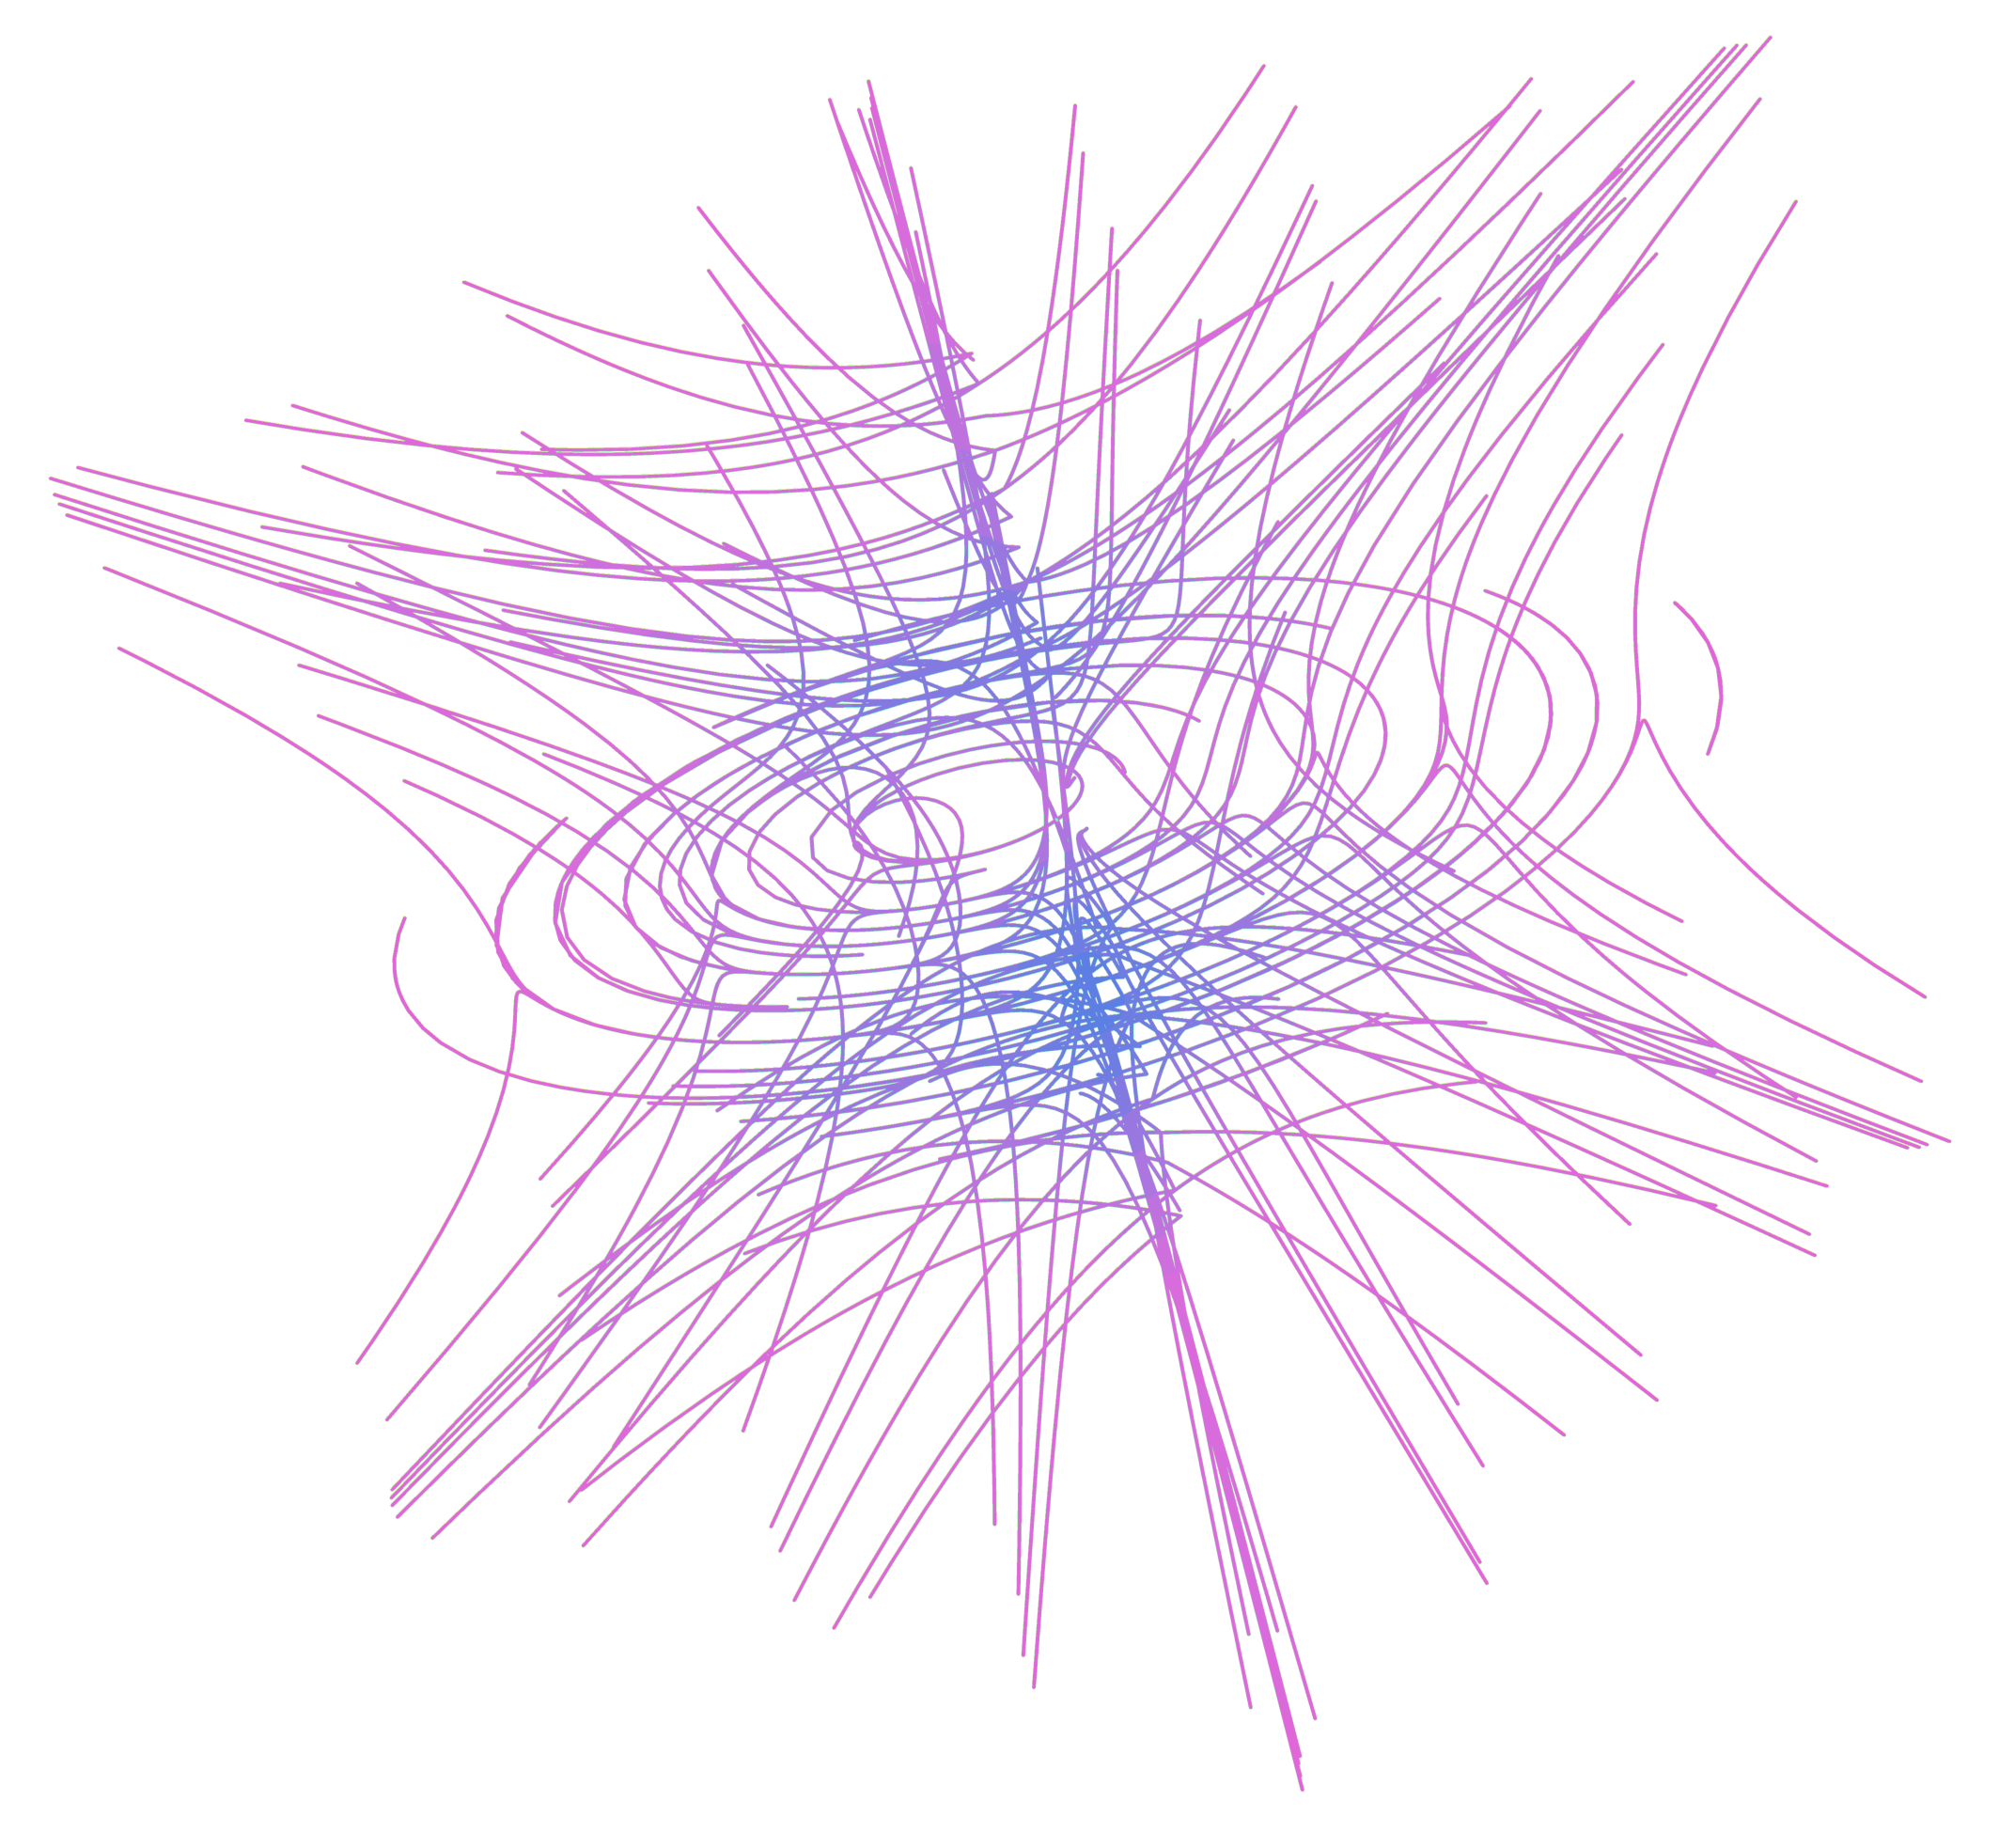
\includegraphics[trim=5cm 5cm 4cm 4cm,width=\paperwidth,height=\paperheight]{../Art/whirl_001_colorised.pdf}}}
\frame[plain]{\titlepage}
}

% Frame 3
% \frame[plain]{\tableofcontents }

\begin{frame}
  \begin{definition}[Harmonic vector field]
    Let $X\subset\R^d$ be a suitable domain.
    A function $f\colon X\to\R$ is \emph{harmonic} if it satisfies the equation
    \begin{align*}
      0=\Delta f=\sum_j\partial_j^2f\,.
    \end{align*}
    A vector field $u\colon X\to\R^d$ is \emph{harmonic} if it is locally the gradient of a harmonic function, that is locally $u=\nabla f$.
  \end{definition}
\end{frame}

\section{Introduction}
{
  % \usebackgroundtemplate{%
  % {\transparent{0.6}\includegraphics[trim=2cm 3cm 5cm -30cm,width=\paperwidth,height=\paperheight]{../Art/centering_003_colorised_fade.pdf}}}
  % {\transparent{0.4}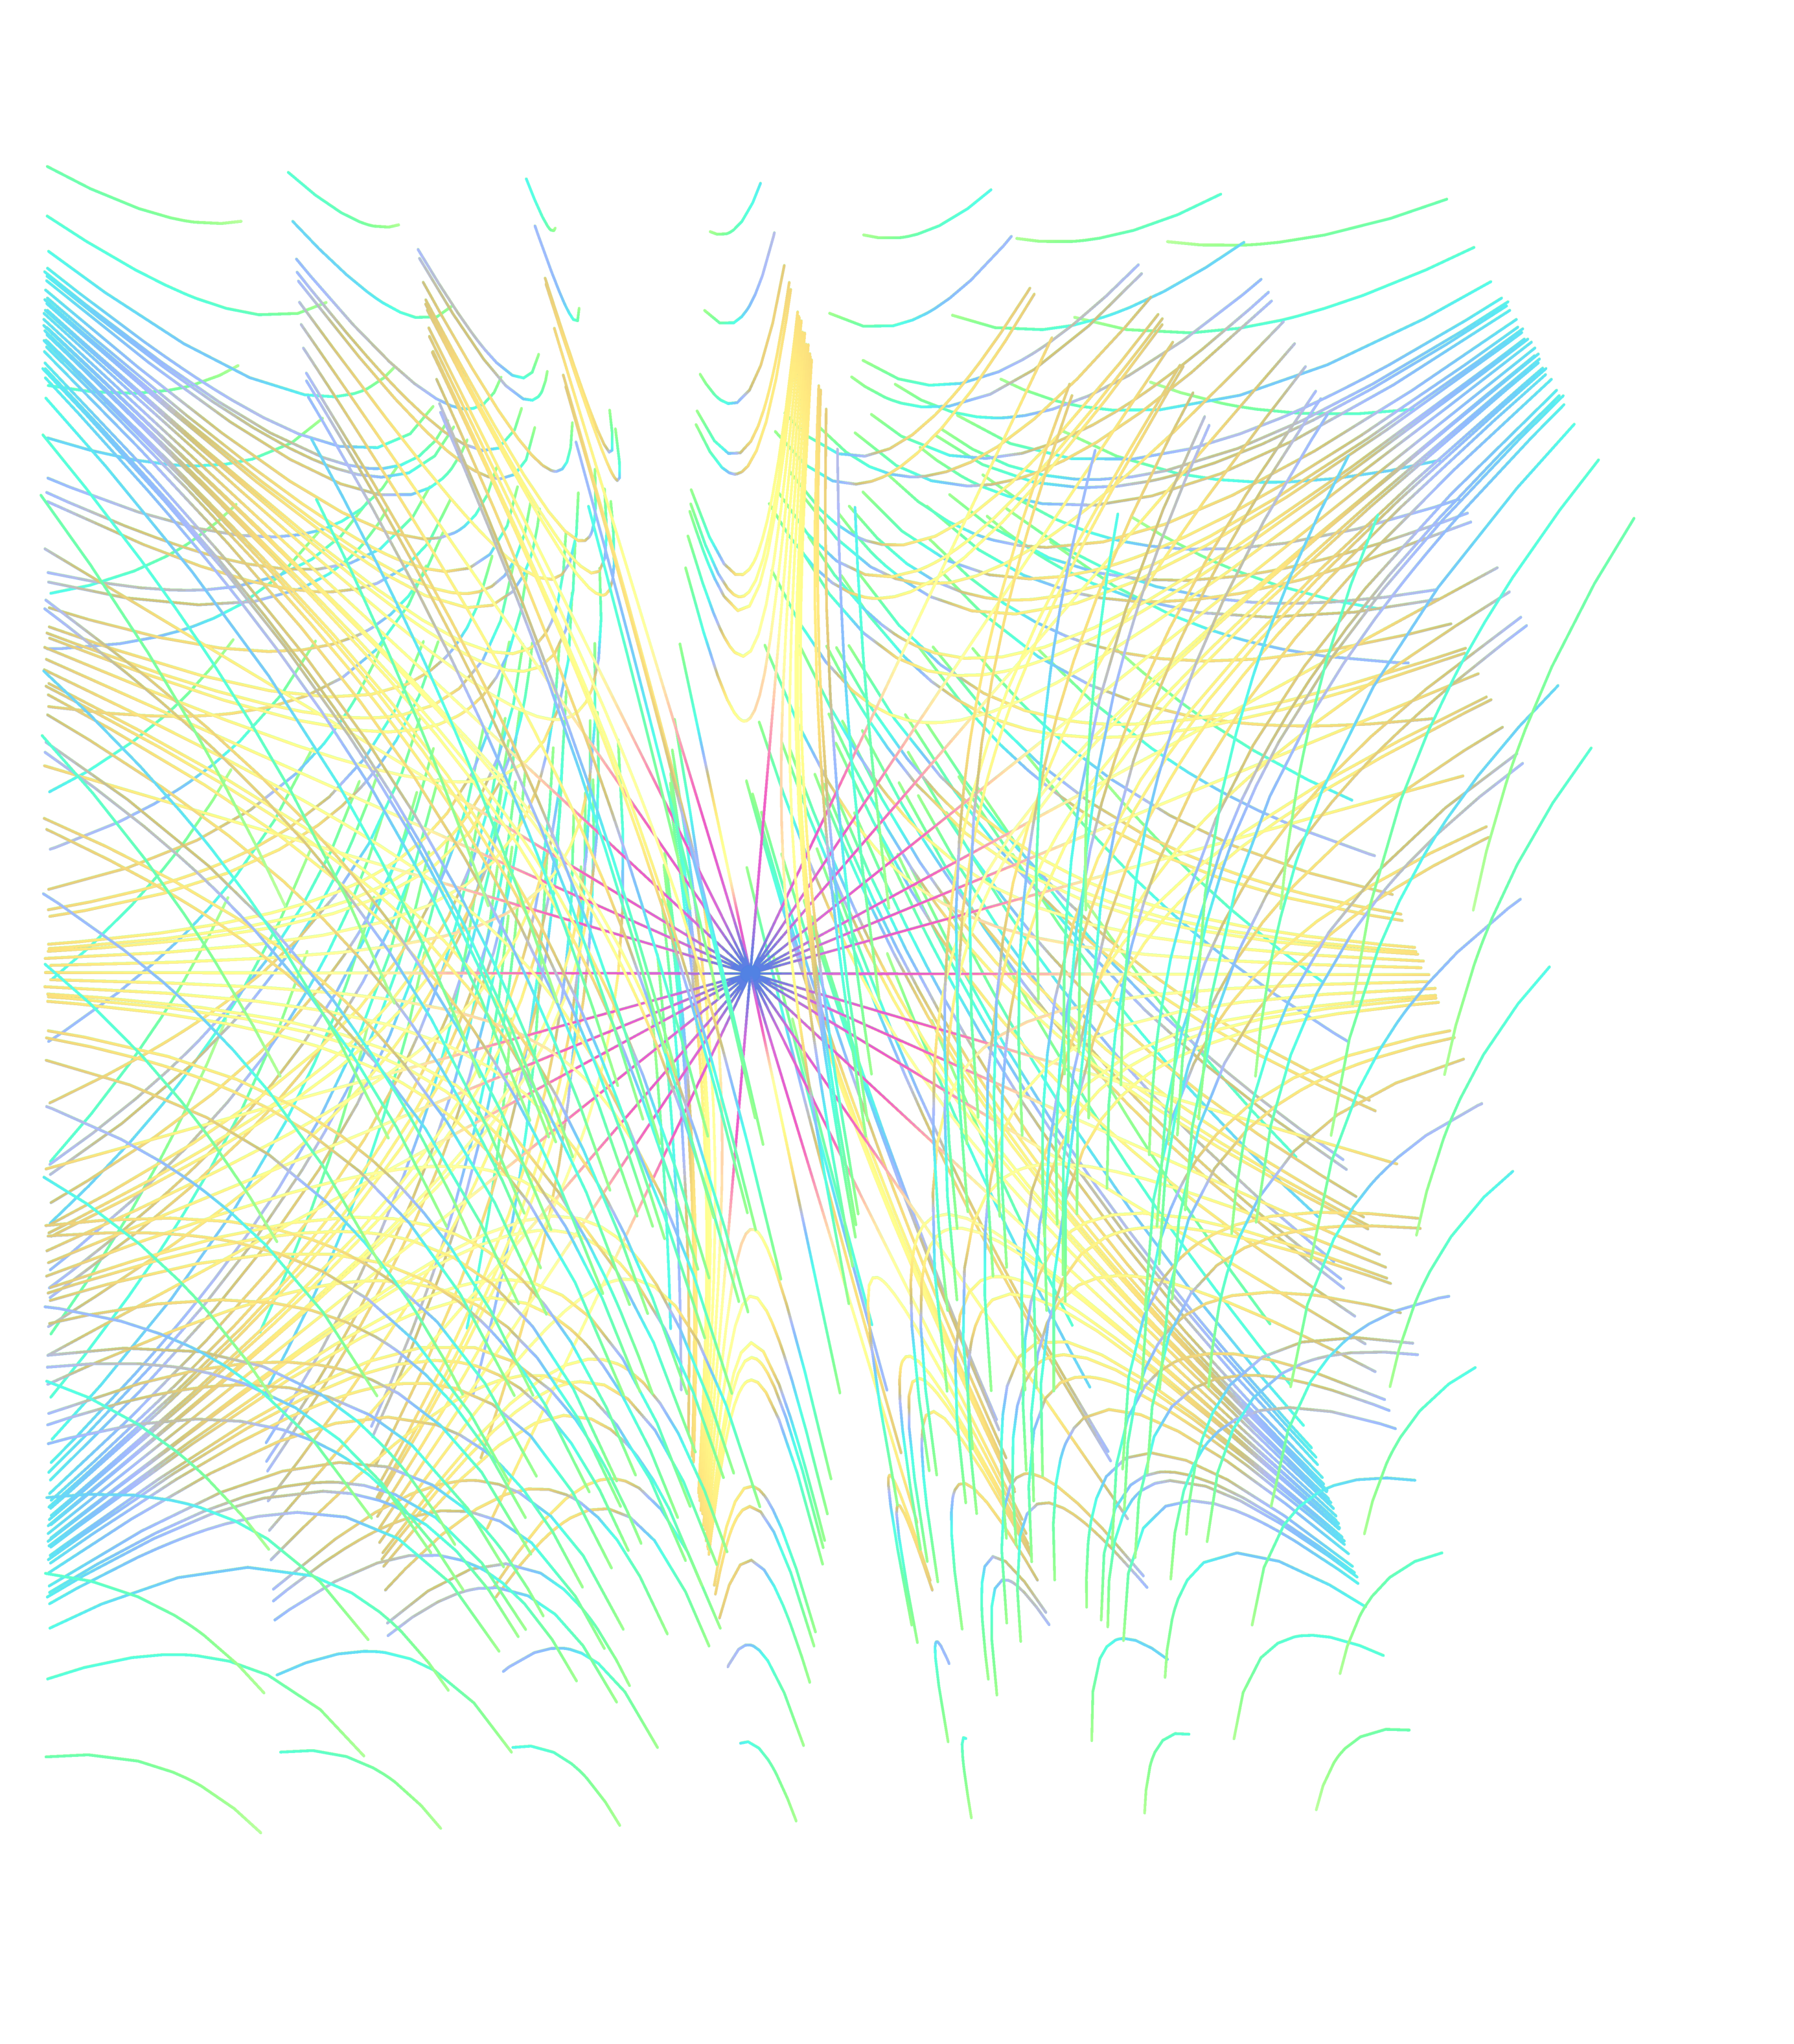
\includegraphics[trim=2cm 15cm 10cm 10cm,width=\paperwidth,height=\paperheight]{../Art/centering_003_colorised.pdf}}}
\begin{frame}[fragile]
  % \frametitle{Why harmonic vector fields?}
  \begin{block}{Why harmonic vector fields?}
    \begin{itemize}
      \item gravitational field in classical mechanics
      \item steady state heat flow
      \item irrotational flow of an inviscid incompressible medium
      \item electrostatic field in vacuum
      \item magnetostatic field in vacuum
    \end{itemize}
  \end{block}
\end{frame}
}

\begin{frame}[fragile]
  \begin{definition}[Stagnation point]
    We call the zeros of a vector field $u\colon X\to\R^d$ \emph{stagnation points}.
    The stagnation points of $u=\nabla f$ are called \emph{critical points} of $f\colon X\to\R$.
  \end{definition}
  \begin{block}{Why stagnation points?}
    \tikzset{external/export=false}
    \[\begin{tikzcd}[column sep=huge]
      \text{vector field topology} \arrow[r,leftrightarrow,"\text{Morse theory}"] &\text{stagnation points}
    \end{tikzcd}\]
  \end{block}
  
\end{frame}

\section{Flowthrough with stagnation point}

\begin{frame}
  The following question is inspired by \autocite["Existence of threedimensional, steady, inviscid,
  incompressible flows with nonvanishing vorticity"]{Alber1992}:
  \questionFlowthrough
\end{frame}

\begin{frame}

  {\transparent{0.6}{\questionFlowthrough}}
  \begin{answer}
    \begin{itemize}
      \item For $d=2$ dimensions: Not possible, see \autocite[Prop. 4.1]{Koppenhoefer2024}.
        The proof uses Morse theory but one can also see this with the argument principle from complex analysis.
    \end{itemize}
  \end{answer}
\end{frame}

\begin{frame}
  \begin{figure}
    \centering
    % \def\svgwidth{\textwidth}
    \scalebox{0.7}{\input{../Figures/n2_cutOmega_corneredMf.pdf_tex}}
    \caption{Idea of the proof involving Morse theory.}
  \end{figure}
\end{frame}


\begin{frame}
  But if one allows for holes in $d=2$ dimensions it becomes possible.
  \begin{figure}
    \centering
    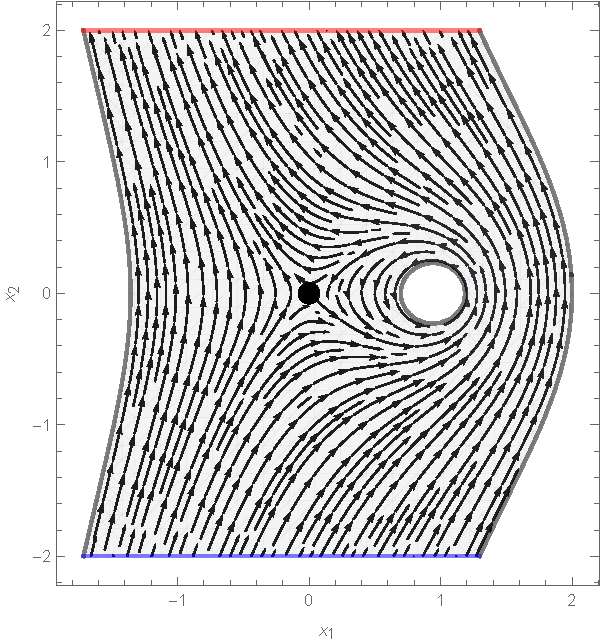
\includegraphics[width=0.5\textwidth]{../Plots/n2_hvf_InflowOutflow_asymmetric_gray_2.pdf}
    % 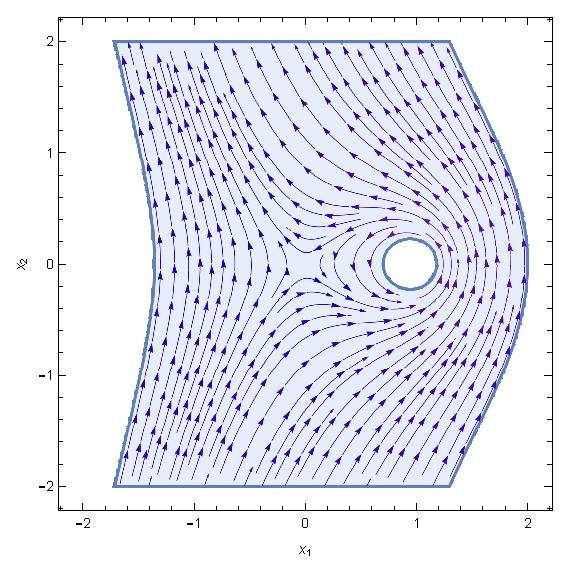
\includegraphics[width=0.6\textwidth]{../Plots/HarmonicVectorFields_gr3.eps}
    \caption{A plot of $u=\nabla^\perp\psi$ in the region $\psi^{-1}\brk*{[-0.5,2]}\cap \brk*{\R\times[-2,2]}$.
    Here $\psi\leftdef\Phi_2\brk*{x-e_1}+x_1$.}
    \label{pl:n2_hvf_InflowOutflow_asymmetric_single}
  \end{figure}
\end{frame}

% \begin{frame}
%  \begin{figure}
%     \centering
%     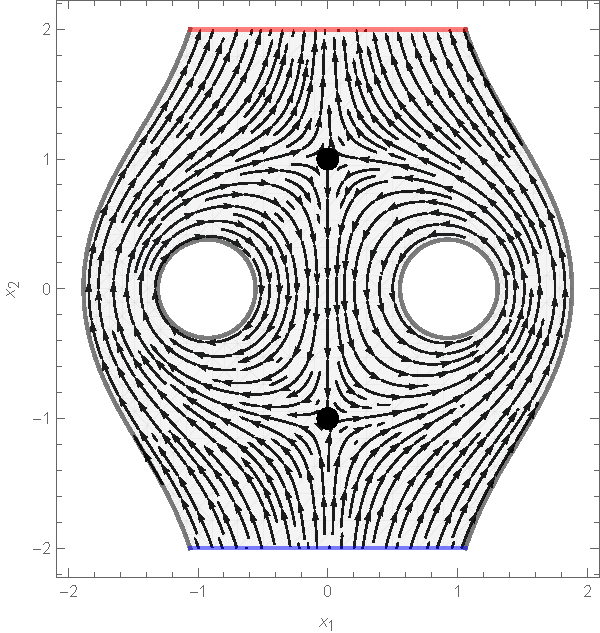
\includegraphics[width=0.6\textwidth]{../Plots/n2_hvf_InflowOutflow_symmetric_gray_2.pdf}
%     % 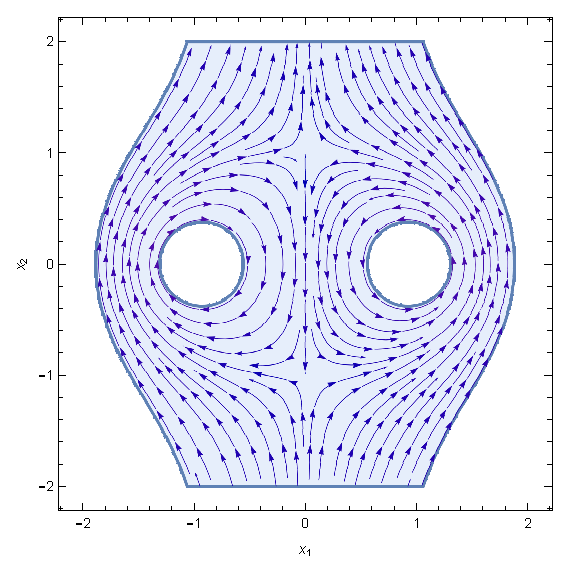
\includegraphics[width=0.6\textwidth]{../Plots/HarmonicVectorFields_gr2.eps}
%     \caption{A plot of $u=\nabla^\perp\psi$ in the region $\psi^{-1}\brk*{[-0.7,0.7]}\cap \brk*{\R\times[-2,2]}$.
%     Here $\psi\leftdef\Phi_2\brk*{x-e_1}-\Phi_2\brk*{x+e_1}+x_1$.} 
%     \label{pl:n2_hvf_InflowOutflow_symmetric_region}
%   \end{figure} 
% \end{frame}

\begin{frame}

  {\transparent{0.6}\questionFlowthrough
  \begin{answer}
    \begin{itemize}
      \item For $d=2$ dimensions: No. 
        {\transparent{1}\item For $d=2$ dimensions for a domain with holes: Possible.}
    \end{itemize}
  \end{answer}}
\end{frame}

\begin{frame}
  \begin{proposition}[Negative answer for cylinders, {\autocite[Prop.\ 5.1]{Koppenhoefer2024}}]\label{pr:n3_inflowOutflowCylinder}
    Let $X=[0,1]\times \overline{U}\subset\R^d$ be a cylinder where $U\subset\R^{d-1}$ is a bounded open set with $C^1$ boundary.
    Let further $f\colon X\to\R$ be non-constant and
    harmonic such that the sides
    $[0,1]\times \partial U=\Sigma^0$ are the tangential boundary,
    the lid $\brk[c]{0}\times U=\Sigma^{\leq0}$ is the entrant boundary and
    the lid $\brk[c]{1}\times U=\Sigma^{\geq0}$ is the emergent boundary. 
    Then $f$ cannot have an interior critical point.
  \end{proposition}
  \begin{proof}
    See blackboard or \autocite{Koppenhoefer2024}.
  \end{proof}
\end{frame}

\begin{frame}
  \begin{figure}
    \centering
    \input{../Figures/n3_cylinder.pdf_tex}
    \caption{This kind of situation is not possible.}
    \label{fi:n3_cylinder}
  \end{figure}
\end{frame}

\begin{frame}

  {\transparent{0.6}\questionFlowthrough
  \begin{answer}
    \begin{itemize}
      \item For $d=2$ dimensions: No.
      \item For $d=2$ dimensions for a domain with holes: Possible.
        {\transparent{1}\item For the cylinder: No.}
    \end{itemize}
  \end{answer}}
\end{frame}

\begin{frame}
  \begin{example}[Connected entrant boundary in $d=4$ dimensions, {\autocite[Ex.\ 4.7]{Koppenhoefer2024}}]\label{ex:n4}
    Consider as domain $X=B_1\subset\R^4$ the unit ball and
    the harmonic function 
    \begin{equation*}
      \begin{aligned}
      f\colon X&\to \R \\
      x &\mapsto x_1^2+x_2^2-x_3^2-x_4^2\,.
      \end{aligned}
      \label{eq:n4_deff}
    \end{equation*}
    This has a critical point at the origin.
    It is shown in \autocite[Prop.\ 4.8]{Koppenhoefer2024} that the entrant and emergent boundaries are in fact connected.
  \end{example} 
\end{frame}

\begin{frame}

  {\transparent{0.6}\questionFlowthrough
  \begin{answer}
    \begin{itemize}
      \item For $d=2$ dimensions: No.
      \item For $d=2$ dimensions for a domain with holes: Possible.
      \item For the cylinder: No.
        {\transparent{1}\item In $d=4$ dimensions: Yes.}
    \end{itemize}
  \end{answer}}
\end{frame}


{
  \usebackgroundtemplate{%
  {\transparent{0.6}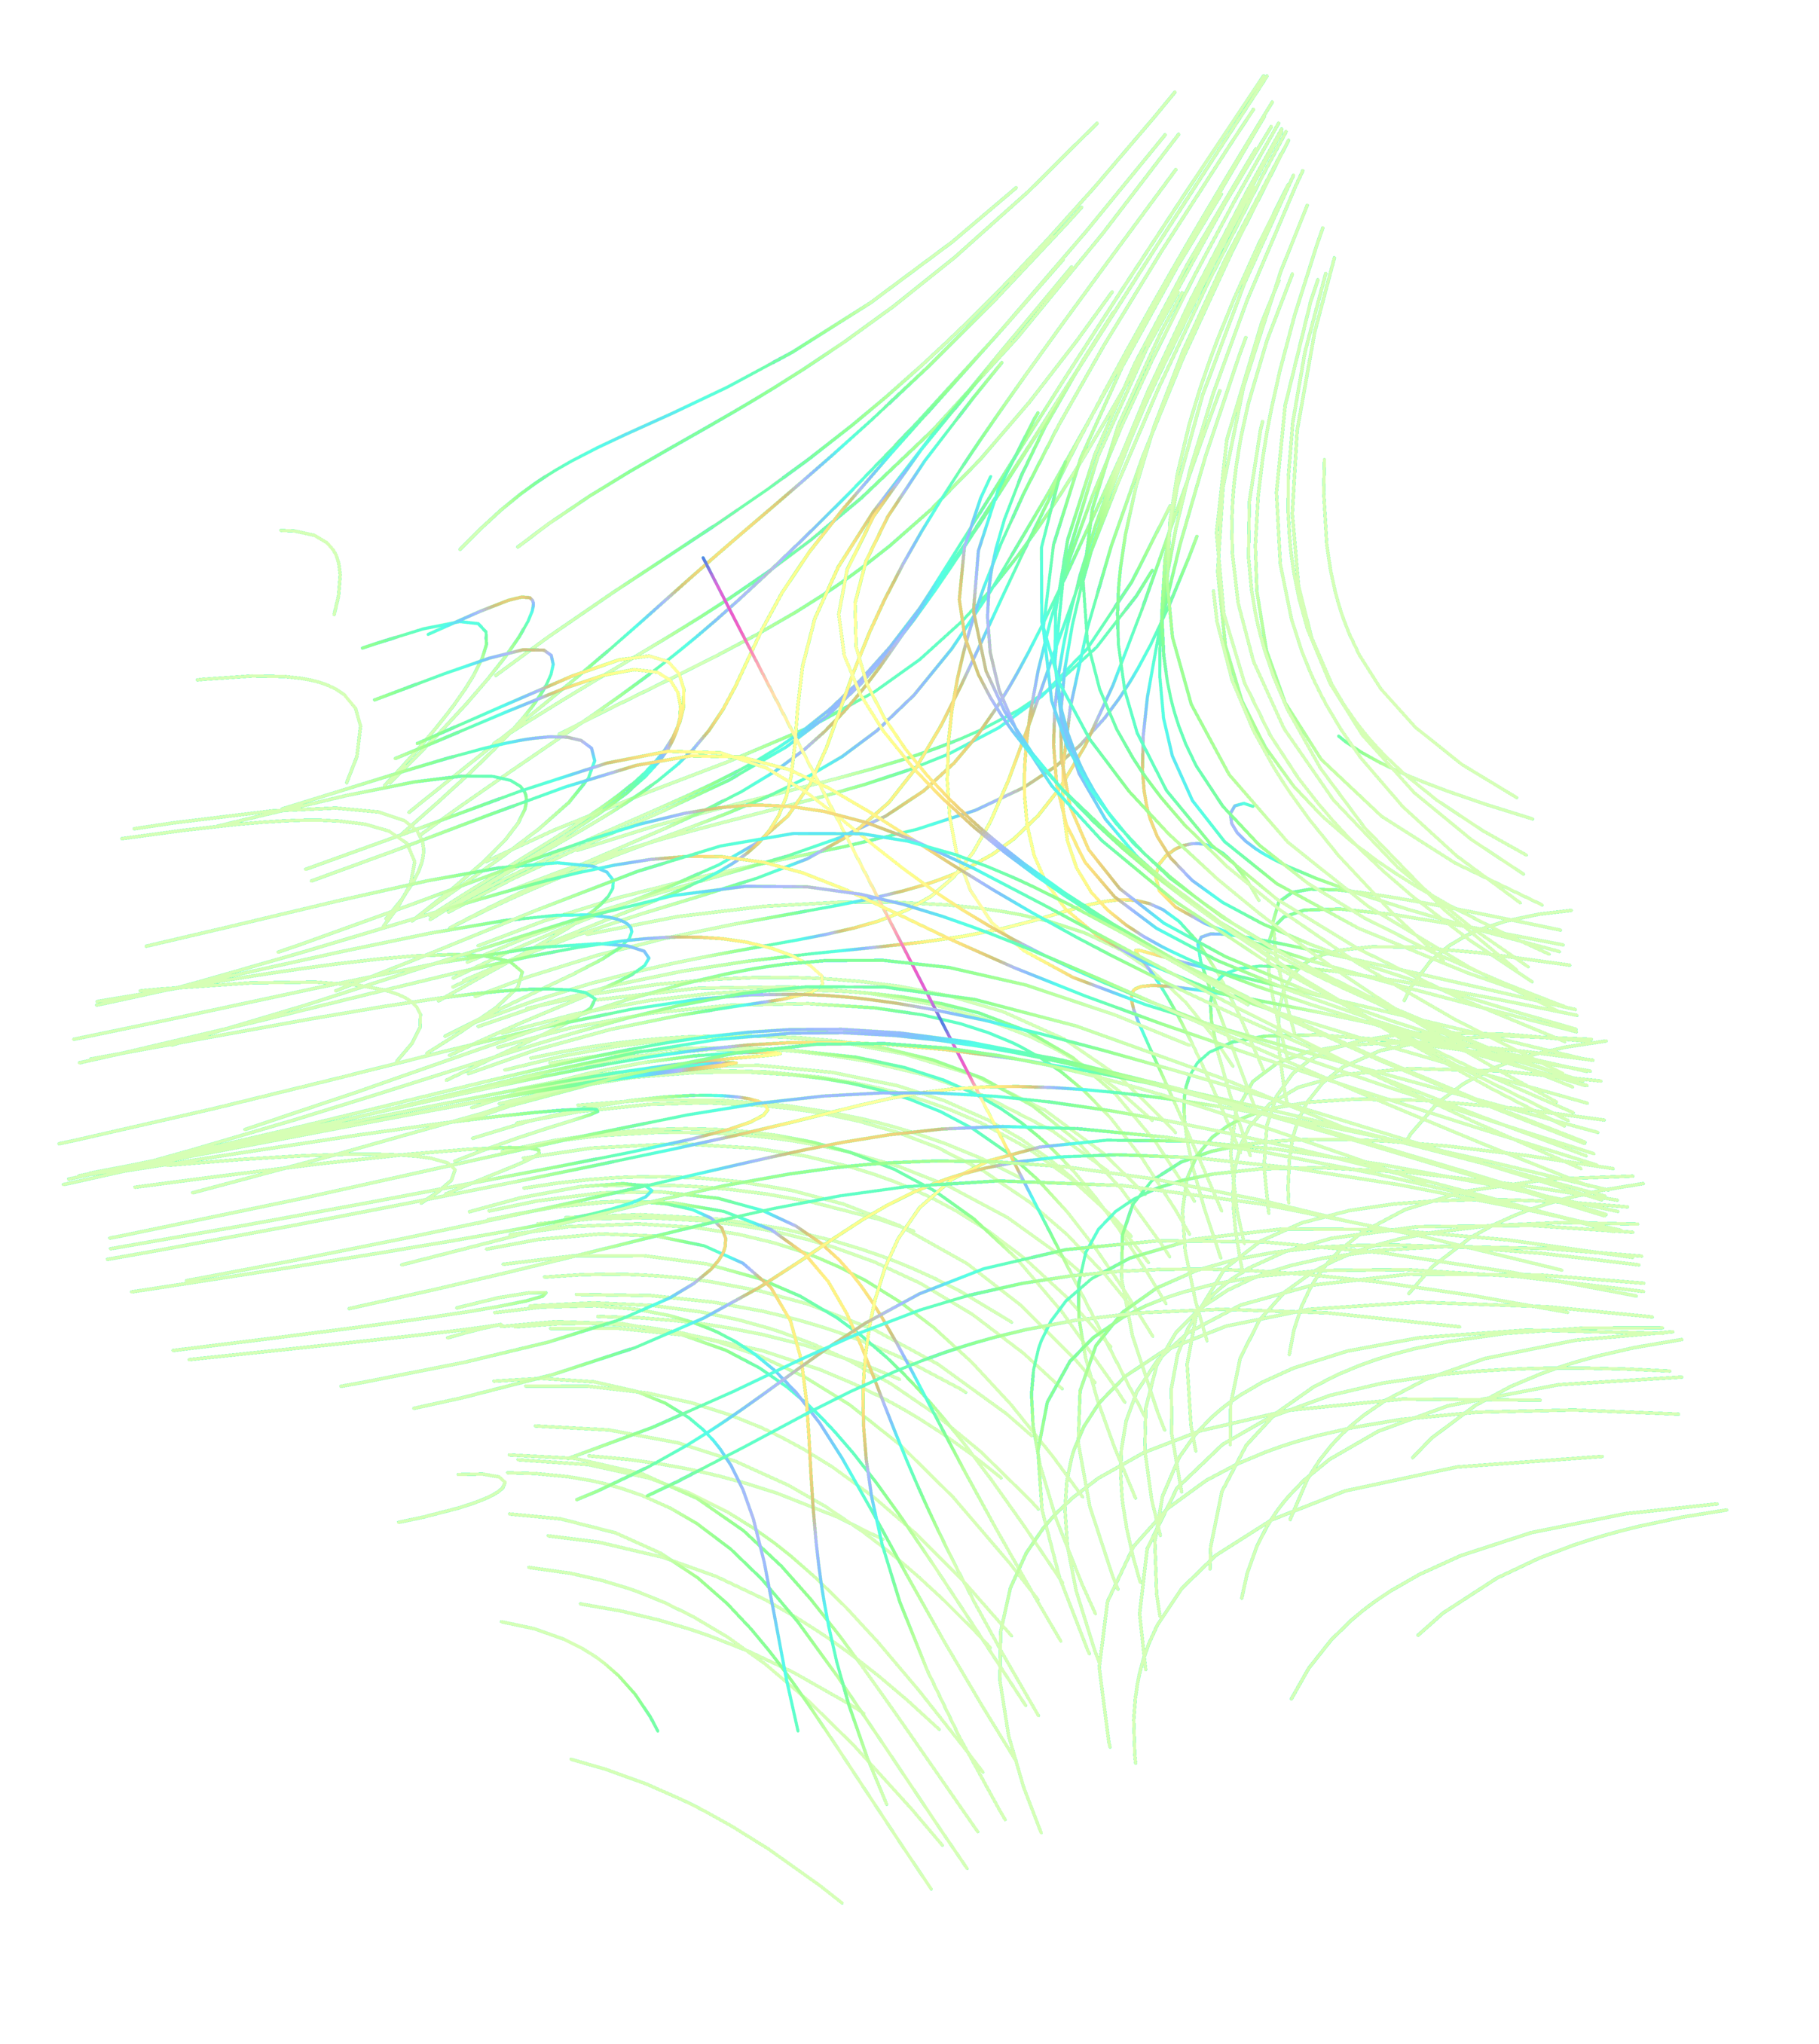
\includegraphics[trim=2cm 5cm 4cm 4cm,width=\paperwidth,height=\paperheight]{../Art/mainExample_005_colorised.pdf}}}
\begin{frame}[plain]
	\begin{center}
    \Large{{So what about $d=3$ dimensions?}}
	\end{center}
\end{frame}
}

\begin{frame}
  \begin{definition}[Interior type numbers]
    Let $u\colon X\to\R^d$ be a vector field and $x$ an interior stagnation point of $u$.
    We say that $x$ is \emph{non-degenerate} if the derivative $Du(x)$ is bijective.
    If in addition $u$ is irrotational we say that $x$ has \emph{Morse index $k$} if $Du(x)$ has exactly $k$ negative eigenvalues.
    The \emph{interior type number} $M_k$ denotes the number of interior stagnation points of index $k$.
  \end{definition}
\end{frame}

\begin{frame}
  \begin{example}[Interior type numbers]
    Consider the harmonic function $f=x_1^2+x_2^2-x_3^2-x_4^2$. One calculates
    \begin{align*}
      u=\nabla f = 2\vect{x_1 & x_2 & -x_3 & -x_4}^\top
    \end{align*}
    which has the sole stagnation point $x=0$. Furthermore
    \begin{align*}
      Du=2\begin{bmatrix}
        1 & & & \\
          & 1 & & \\
          & & -1 & \\
          & & & -1
      \end{bmatrix}
    \end{align*}
    which implies that $x=0$ is non-degenerate and has Morse index $2$.
    This implies $M_2=1$ and $M_k=0$ for $k\neq2$.
  \end{example}
\end{frame}


\begin{frame}
  \begin{proposition}[Condition on the interior type numbers, {\autocite[Prop.\ 5.2]{Koppenhoefer2024}}]\label{pr:n3_inflowOutflowRels}
    Let $X\subset\R^3$ be a compact three-dimensional manifold with corners and
    let $f\colon X\to\R$ be a harmonic function without irregular stagnation points and such that $f$ is non-degenerate on the interior $\interior\brk*{X}$.
    Let $\Sigma=\Sigma_{\leq0}\sqcup\Sigma_{\geq0}$ be a disjoint decomposition of the boundary into simply connected nonempty sets such that
    we have for the strictly entrant boundary $\Sigma^-\subseteq\Sigma_{\leq0}$ and for the strictly emergent boundary
    $\Sigma^+\subseteq\Sigma_{\geq0}$. Additionally we require that $\gamma\leftdef\partial\Sigma_{\leq0}$ is a one-dimensional manifold diffeomorphic to the
    circle $S^1$.
    Then we have the relation $M_1=M_2$ between the interior type numbers.
  \end{proposition}
\end{frame}

\begin{frame}

  {\transparent{0.6}\questionFlowthrough
  \begin{answer}
    \begin{itemize}
      \item For $d=2$ dimensions: No.
      \item For $d=2$ dimensions for a domain with holes: Possible.
      \item For the cylinder: No.
      \item In $d=4$ dimensions: Yes.
        {\transparent{1}\item In $d=3$ dimensions: Has to have an even number of stagnation points.}
    \end{itemize}
  \end{answer}}
\end{frame}

\begin{frame}
  \begin{example}[A harmonic function with interior critical points and connected entrant and emergent boundaries, {\autocite[Ex.\ 5.3]{Koppenhoefer2024}}]
    For $d=3$ dimensions we have for $r$ sufficiently large the example $X=B_r$, $u=\nabla f$ with
    \begin{align*}
      f=\frac{x_1^2}{2}-\frac{x_1^3}{3}-\frac{x_1x_2^2}{2}+x_1x_2^2+x_2x_3\,.
    \end{align*}
    This is
    \begin{itemize}
      \item harmonic
      \item has critical points at $0$ and $e_1$
      \item connected entrant and emergent boundaries.
    \end{itemize}
    
  \end{example}
\end{frame}

\begin{frame}
  \begin{figure}
    \centering
    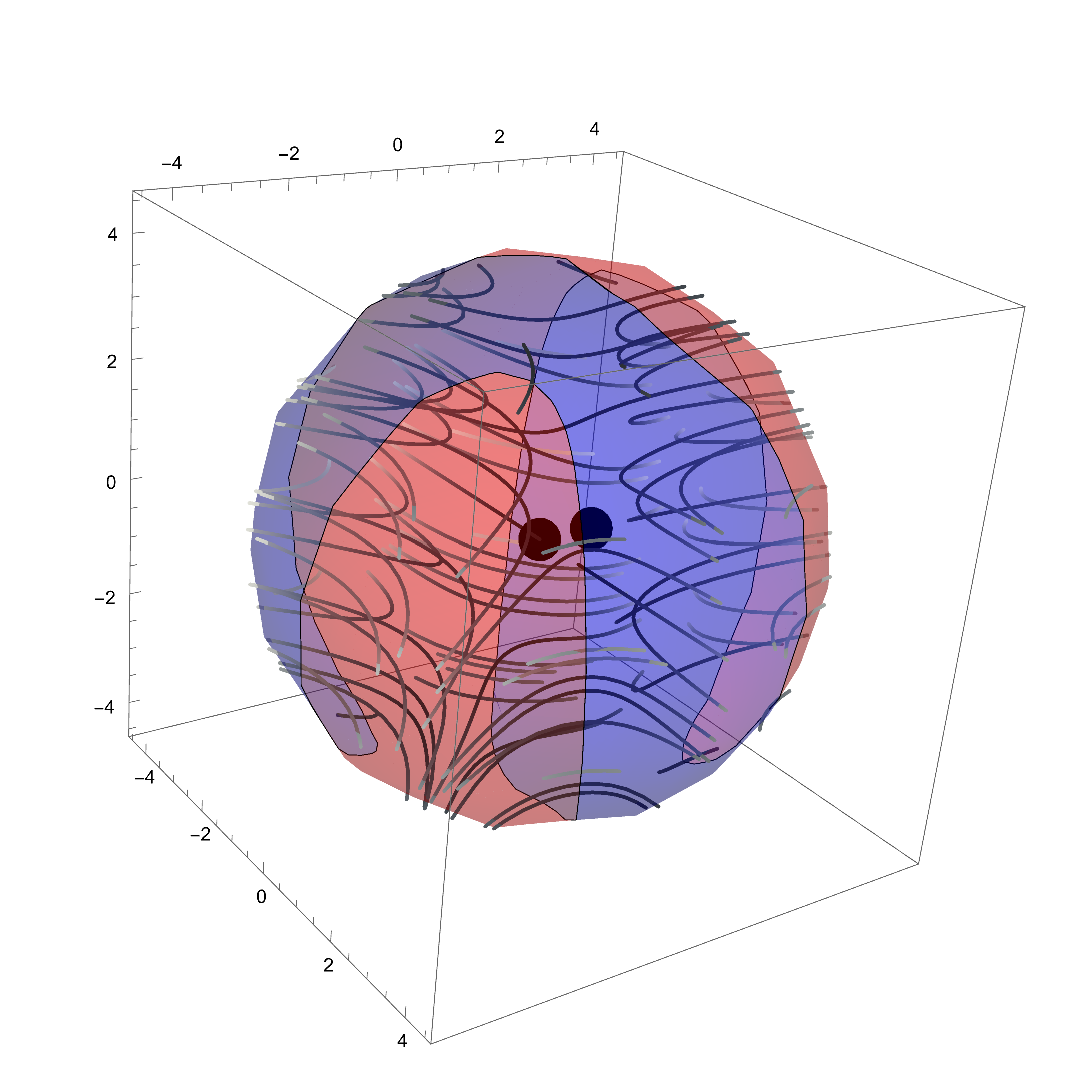
\includegraphics[width=0.6\textwidth]{../plots/n3_hf_inflowOutflow_Ball_overview.pdf}
    \caption{A stream plot of the function $u$. The interior stagnation points are highlighted in black.
    $\Sigma^+$ is shaded red, $\Sigma^-$ blue.}
    \label{pl:n3_hf_inflowOutflowStagnationPoint_overview}
  \end{figure}
\end{frame}

\begin{frame}
  \begin{figure}
    \centering
    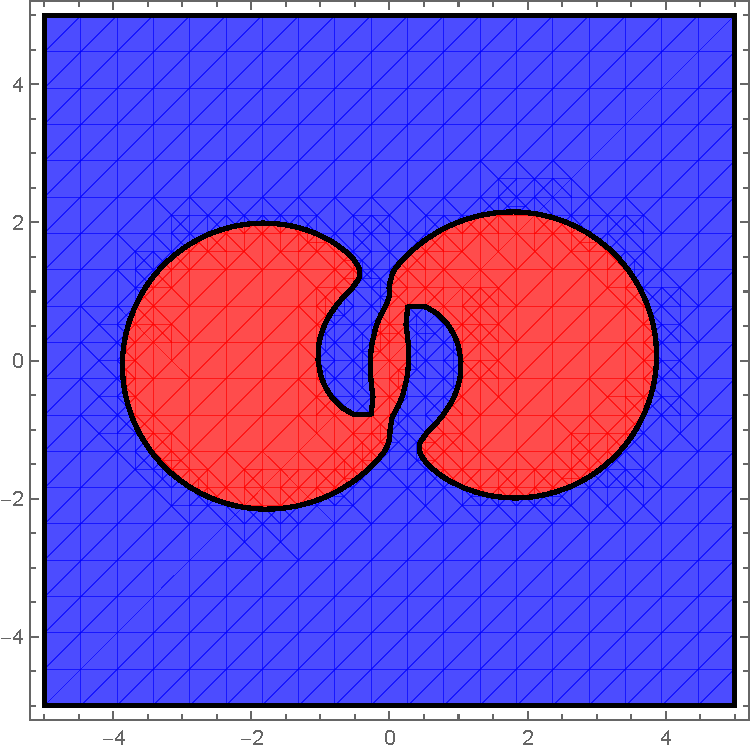
\includegraphics[width=0.6\textwidth]{../plots/n3_hf_inflowOutflow_Ball_Surface_2.pdf}
    \caption{Stereographic projection of the surface $\Sigma$. $\Sigma^+$ is shaded red, $\Sigma^-$ blue.}
    \label{pl:n3_hf_inflowOutflowStagnationPoint_Surface}
  \end{figure}
\end{frame}

% \begin{frame}[fragile]
%   Let $\e=1/r$ and
%   let $\cV_\e$ be the curve separating $\Sigma^+$ and $\Sigma^-$ projected onto $B_1$. 
%   \begin{center}
%     \tikzset{external/export next=false}
%     \begin{tikzcd}[sep=small]
%       \text{Smoothness of }\cV_\e \arrow[dr]\arrow[rr] & & \text{Connectedness of }\cV_\e \arrow[ld] \\
%                                                        & \parbox{4cm}{Regions $\Sigma^+$ and $\Sigma^-$ are connected} & 
%   \end{tikzcd}
%   
%   \end{center}
% \end{frame}

\begin{frame}
  Let $\e=1/r$ and
  let $r\cV_\e$ be the curve separating $\Sigma^+$ and $\Sigma^-$. 
  \begin{figure}
    \centering
    \resizebox{\textwidth}{!}{
      % Graphic for TeX using PGF
% Title: Proof_solution.dia
% Creator: Dia v0.97+git
% CreationDate: Tue Apr 16 14:47:52 2024
% For: theo
% \usepackage{tikz}
% The following commands are not supported in PSTricks at present
% We define them conditionally, so when they are implemented,
% this pgf file will use them.
\ifx\du\undefined
  \newlength{\du}
\fi
\setlength{\du}{15\unitlength}
\begin{tikzpicture}[even odd rule]
\pgftransformxscale{1.000000}
\pgftransformyscale{-1.000000}
\definecolor{dialinecolor}{rgb}{0.000000, 0.000000, 0.000000}
\pgfsetstrokecolor{dialinecolor}
\pgfsetstrokeopacity{1.000000}
\definecolor{diafillcolor}{rgb}{1.000000, 1.000000, 1.000000}
\pgfsetfillcolor{diafillcolor}
\pgfsetfillopacity{1.000000}
\pgfsetlinewidth{0.100000\du}
\pgfsetdash{}{0pt}
\pgfsetmiterjoin
{\pgfsetcornersarced{\pgfpoint{0.000000\du}{0.000000\du}}\definecolor{diafillcolor}{rgb}{1.000000, 1.000000, 1.000000}
\pgfsetfillcolor{diafillcolor}
\pgfsetfillopacity{1.000000}
\fill (7.150150\du,10.912100\du)--(7.150150\du,13.612100\du)--(15.957650\du,13.612100\du)--(15.957650\du,10.912100\du)--cycle;
}{\pgfsetcornersarced{\pgfpoint{0.000000\du}{0.000000\du}}\definecolor{dialinecolor}{rgb}{0.000000, 0.000000, 0.000000}
\pgfsetstrokecolor{dialinecolor}
\pgfsetstrokeopacity{1.000000}
\draw (7.150150\du,10.912100\du)--(7.150150\du,13.612100\du)--(15.957650\du,13.612100\du)--(15.957650\du,10.912100\du)--cycle;
}% setfont left to latex
\definecolor{dialinecolor}{rgb}{0.000000, 0.000000, 0.000000}
\pgfsetstrokecolor{dialinecolor}
\pgfsetstrokeopacity{1.000000}
\definecolor{diafillcolor}{rgb}{0.000000, 0.000000, 0.000000}
\pgfsetfillcolor{diafillcolor}
\pgfsetfillopacity{1.000000}
\node[anchor=base,inner sep=0pt, outer sep=0pt,color=dialinecolor] at (11.553900\du,12.056163\du){Smoothness of $\cV_\e$};
% setfont left to latex
\definecolor{dialinecolor}{rgb}{0.000000, 0.000000, 0.000000}
\pgfsetstrokecolor{dialinecolor}
\pgfsetstrokeopacity{1.000000}
\definecolor{diafillcolor}{rgb}{0.000000, 0.000000, 0.000000}
\pgfsetfillcolor{diafillcolor}
\pgfsetfillopacity{1.000000}
\node[anchor=base,inner sep=0pt, outer sep=0pt,color=dialinecolor] at (11.553900\du,12.856163\du){(Lemma 5.6)};
\pgfsetlinewidth{0.100000\du}
\pgfsetdash{}{0pt}
\pgfsetmiterjoin
{\pgfsetcornersarced{\pgfpoint{0.000000\du}{0.000000\du}}\definecolor{diafillcolor}{rgb}{1.000000, 1.000000, 1.000000}
\pgfsetfillcolor{diafillcolor}
\pgfsetfillopacity{1.000000}
\fill (17.622700\du,10.918300\du)--(17.622700\du,13.618300\du)--(27.410200\du,13.618300\du)--(27.410200\du,10.918300\du)--cycle;
}{\pgfsetcornersarced{\pgfpoint{0.000000\du}{0.000000\du}}\definecolor{dialinecolor}{rgb}{0.000000, 0.000000, 0.000000}
\pgfsetstrokecolor{dialinecolor}
\pgfsetstrokeopacity{1.000000}
\draw (17.622700\du,10.918300\du)--(17.622700\du,13.618300\du)--(27.410200\du,13.618300\du)--(27.410200\du,10.918300\du)--cycle;
}% setfont left to latex
\definecolor{dialinecolor}{rgb}{0.000000, 0.000000, 0.000000}
\pgfsetstrokecolor{dialinecolor}
\pgfsetstrokeopacity{1.000000}
\definecolor{diafillcolor}{rgb}{0.000000, 0.000000, 0.000000}
\pgfsetfillcolor{diafillcolor}
\pgfsetfillopacity{1.000000}
\node[anchor=base,inner sep=0pt, outer sep=0pt,color=dialinecolor] at (22.516450\du,12.062363\du){Connectedness of $\cV_\e$};
% setfont left to latex
\definecolor{dialinecolor}{rgb}{0.000000, 0.000000, 0.000000}
\pgfsetstrokecolor{dialinecolor}
\pgfsetstrokeopacity{1.000000}
\definecolor{diafillcolor}{rgb}{0.000000, 0.000000, 0.000000}
\pgfsetfillcolor{diafillcolor}
\pgfsetfillopacity{1.000000}
\node[anchor=base,inner sep=0pt, outer sep=0pt,color=dialinecolor] at (22.516450\du,12.862363\du){(Lemma 5.9)};
\pgfsetlinewidth{0.100000\du}
\pgfsetdash{}{0pt}
\pgfsetmiterjoin
{\pgfsetcornersarced{\pgfpoint{0.000000\du}{0.000000\du}}\definecolor{diafillcolor}{rgb}{1.000000, 1.000000, 1.000000}
\pgfsetfillcolor{diafillcolor}
\pgfsetfillopacity{1.000000}
\fill (10.290700\du,18.175800\du)--(10.290700\du,20.875800\du)--(23.645700\du,20.875800\du)--(23.645700\du,18.175800\du)--cycle;
}{\pgfsetcornersarced{\pgfpoint{0.000000\du}{0.000000\du}}\definecolor{dialinecolor}{rgb}{0.000000, 0.000000, 0.000000}
\pgfsetstrokecolor{dialinecolor}
\pgfsetstrokeopacity{1.000000}
\draw (10.290700\du,18.175800\du)--(10.290700\du,20.875800\du)--(23.645700\du,20.875800\du)--(23.645700\du,18.175800\du)--cycle;
}% setfont left to latex
\definecolor{dialinecolor}{rgb}{0.000000, 0.000000, 0.000000}
\pgfsetstrokecolor{dialinecolor}
\pgfsetstrokeopacity{1.000000}
\definecolor{diafillcolor}{rgb}{0.000000, 0.000000, 0.000000}
\pgfsetfillcolor{diafillcolor}
\pgfsetfillopacity{1.000000}
\node[anchor=base,inner sep=0pt, outer sep=0pt,color=dialinecolor] at (16.968200\du,19.319862\du){Regions $\Sigma^+$ and $\Sigma^-$};
% setfont left to latex
\definecolor{dialinecolor}{rgb}{0.000000, 0.000000, 0.000000}
\pgfsetstrokecolor{dialinecolor}
\pgfsetstrokeopacity{1.000000}
\definecolor{diafillcolor}{rgb}{0.000000, 0.000000, 0.000000}
\pgfsetfillcolor{diafillcolor}
\pgfsetfillopacity{1.000000}
\node[anchor=base,inner sep=0pt, outer sep=0pt,color=dialinecolor] at (16.968200\du,20.119862\du){are connected (Theorem 5.4)};
\pgfsetlinewidth{0.100000\du}
\pgfsetdash{}{0pt}
\pgfsetmiterjoin
\pgfsetbuttcap
{
\definecolor{diafillcolor}{rgb}{0.000000, 0.000000, 0.000000}
\pgfsetfillcolor{diafillcolor}
\pgfsetfillopacity{1.000000}
% was here!!!
\pgfsetarrowsend{stealth}
{\pgfsetcornersarced{\pgfpoint{0.000000\du}{0.000000\du}}\definecolor{dialinecolor}{rgb}{0.000000, 0.000000, 0.000000}
\pgfsetstrokecolor{dialinecolor}
\pgfsetstrokeopacity{1.000000}
\draw (11.553900\du,13.612100\du)--(11.553900\du,16.895500\du)--(13.629500\du,16.895500\du)--(13.629500\du,18.175800\du);
}}
\pgfsetlinewidth{0.100000\du}
\pgfsetdash{}{0pt}
\pgfsetmiterjoin
\pgfsetbuttcap
{
\definecolor{diafillcolor}{rgb}{0.000000, 0.000000, 0.000000}
\pgfsetfillcolor{diafillcolor}
\pgfsetfillopacity{1.000000}
% was here!!!
\pgfsetarrowsend{stealth}
{\pgfsetcornersarced{\pgfpoint{0.000000\du}{0.000000\du}}\definecolor{dialinecolor}{rgb}{0.000000, 0.000000, 0.000000}
\pgfsetstrokecolor{dialinecolor}
\pgfsetstrokeopacity{1.000000}
\draw (22.516400\du,13.618300\du)--(22.516400\du,16.927900\du)--(20.307000\du,16.927900\du)--(20.307000\du,18.175800\du);
}}
% setfont left to latex
\definecolor{dialinecolor}{rgb}{0.000000, 0.000000, 0.000000}
\pgfsetstrokecolor{dialinecolor}
\pgfsetstrokeopacity{1.000000}
\definecolor{diafillcolor}{rgb}{0.000000, 0.000000, 0.000000}
\pgfsetfillcolor{diafillcolor}
\pgfsetfillopacity{1.000000}
\node[anchor=base west,inner sep=0pt,outer sep=0pt,color=dialinecolor] at (13.507400\du,15.991000\du){Jordan curve theorem};
\pgfsetlinewidth{0.100000\du}
\pgfsetdash{}{0pt}
\pgfsetmiterjoin
\pgfsetbuttcap
{
\definecolor{diafillcolor}{rgb}{0.000000, 0.000000, 0.000000}
\pgfsetfillcolor{diafillcolor}
\pgfsetfillopacity{1.000000}
% was here!!!
\pgfsetarrowsend{stealth}
{\pgfsetcornersarced{\pgfpoint{0.000000\du}{0.000000\du}}\definecolor{dialinecolor}{rgb}{0.000000, 0.000000, 0.000000}
\pgfsetstrokecolor{dialinecolor}
\pgfsetstrokeopacity{1.000000}
\draw (15.957650\du,12.262100\du)--(16.790175\du,12.262100\du)--(16.790175\du,12.268300\du)--(17.622700\du,12.268300\du);
}}
\end{tikzpicture}

    }
  \end{figure}
\end{frame}

\begin{frame}
  \frametitle{Proof of smoothness (Lemma 5.6)}
  \begin{itemize}
    \item Here smoothness means that $\cV_\e$ is a differentiable manifold \textrightarrow Jacobi criterion
    \item $\cV_\e$ is an algebraic variety \textrightarrow use Gröbner bases to show that Jacobi criterion is fulfilled for sufficiently large $r>0$
  \end{itemize}
\end{frame}


\begin{frame}
  \frametitle{Proof of connectedness (Lemma 5.9)}
  \begin{figure}
    \centering
    \resizebox{\textwidth}{!}{
      % Graphic for TeX using PGF
% Title: Proof_connectedness.dia
% Creator: Dia v0.97+git
% CreationDate: Tue Apr 16 14:47:52 2024
% For: theo
% \usepackage{tikz}
% The following commands are not supported in PSTricks at present
% We define them conditionally, so when they are implemented,
% this pgf file will use them.
\ifx\du\undefined
  \newlength{\du}
\fi
\setlength{\du}{15\unitlength}
\begin{tikzpicture}[even odd rule]
\pgftransformxscale{1.000000}
\pgftransformyscale{-1.000000}
\definecolor{dialinecolor}{rgb}{0.000000, 0.000000, 0.000000}
\pgfsetstrokecolor{dialinecolor}
\pgfsetstrokeopacity{1.000000}
\definecolor{diafillcolor}{rgb}{1.000000, 1.000000, 1.000000}
\pgfsetfillcolor{diafillcolor}
\pgfsetfillopacity{1.000000}
\pgfsetlinewidth{0.100000\du}
\pgfsetdash{}{0pt}
\pgfsetmiterjoin
{\pgfsetcornersarced{\pgfpoint{0.000000\du}{0.000000\du}}\definecolor{diafillcolor}{rgb}{1.000000, 1.000000, 1.000000}
\pgfsetfillcolor{diafillcolor}
\pgfsetfillopacity{1.000000}
\fill (17.988000\du,17.665900\du)--(17.988000\du,20.365900\du)--(27.775500\du,20.365900\du)--(27.775500\du,17.665900\du)--cycle;
}{\pgfsetcornersarced{\pgfpoint{0.000000\du}{0.000000\du}}\definecolor{dialinecolor}{rgb}{0.000000, 0.000000, 0.000000}
\pgfsetstrokecolor{dialinecolor}
\pgfsetstrokeopacity{1.000000}
\draw (17.988000\du,17.665900\du)--(17.988000\du,20.365900\du)--(27.775500\du,20.365900\du)--(27.775500\du,17.665900\du)--cycle;
}% setfont left to latex
\definecolor{dialinecolor}{rgb}{0.000000, 0.000000, 0.000000}
\pgfsetstrokecolor{dialinecolor}
\pgfsetstrokeopacity{1.000000}
\definecolor{diafillcolor}{rgb}{0.000000, 0.000000, 0.000000}
\pgfsetfillcolor{diafillcolor}
\pgfsetfillopacity{1.000000}
\node[anchor=base,inner sep=0pt, outer sep=0pt,color=dialinecolor] at (22.881750\du,18.809963\du){Connectedness of $\cV_\e$};
% setfont left to latex
\definecolor{dialinecolor}{rgb}{0.000000, 0.000000, 0.000000}
\pgfsetstrokecolor{dialinecolor}
\pgfsetstrokeopacity{1.000000}
\definecolor{diafillcolor}{rgb}{0.000000, 0.000000, 0.000000}
\pgfsetfillcolor{diafillcolor}
\pgfsetfillopacity{1.000000}
\node[anchor=base,inner sep=0pt, outer sep=0pt,color=dialinecolor] at (22.881750\du,19.609963\du){(Lemma 5.9)};
\pgfsetlinewidth{0.100000\du}
\pgfsetdash{}{0pt}
\pgfsetmiterjoin
{\pgfsetcornersarced{\pgfpoint{0.000000\du}{0.000000\du}}\definecolor{diafillcolor}{rgb}{1.000000, 1.000000, 1.000000}
\pgfsetfillcolor{diafillcolor}
\pgfsetfillopacity{1.000000}
\fill (6.996250\du,6.699970\du)--(6.996250\du,9.399970\du)--(15.803750\du,9.399970\du)--(15.803750\du,6.699970\du)--cycle;
}{\pgfsetcornersarced{\pgfpoint{0.000000\du}{0.000000\du}}\definecolor{dialinecolor}{rgb}{0.000000, 0.000000, 0.000000}
\pgfsetstrokecolor{dialinecolor}
\pgfsetstrokeopacity{1.000000}
\draw (6.996250\du,6.699970\du)--(6.996250\du,9.399970\du)--(15.803750\du,9.399970\du)--(15.803750\du,6.699970\du)--cycle;
}% setfont left to latex
\definecolor{dialinecolor}{rgb}{0.000000, 0.000000, 0.000000}
\pgfsetstrokecolor{dialinecolor}
\pgfsetstrokeopacity{1.000000}
\definecolor{diafillcolor}{rgb}{0.000000, 0.000000, 0.000000}
\pgfsetfillcolor{diafillcolor}
\pgfsetfillopacity{1.000000}
\node[anchor=base,inner sep=0pt, outer sep=0pt,color=dialinecolor] at (11.400000\du,7.844033\du){Smoothness of $\cV_\e$};
% setfont left to latex
\definecolor{dialinecolor}{rgb}{0.000000, 0.000000, 0.000000}
\pgfsetstrokecolor{dialinecolor}
\pgfsetstrokeopacity{1.000000}
\definecolor{diafillcolor}{rgb}{0.000000, 0.000000, 0.000000}
\pgfsetfillcolor{diafillcolor}
\pgfsetfillopacity{1.000000}
\node[anchor=base,inner sep=0pt, outer sep=0pt,color=dialinecolor] at (11.400000\du,8.644033\du){(Lemma 5.6)};
\pgfsetlinewidth{0.100000\du}
\pgfsetdash{}{0pt}
\pgfsetmiterjoin
{\pgfsetcornersarced{\pgfpoint{0.000000\du}{0.000000\du}}\definecolor{diafillcolor}{rgb}{1.000000, 1.000000, 1.000000}
\pgfsetfillcolor{diafillcolor}
\pgfsetfillopacity{1.000000}
\fill (5.222500\du,17.250000\du)--(5.222500\du,20.750000\du)--(15.677500\du,20.750000\du)--(15.677500\du,17.250000\du)--cycle;
}{\pgfsetcornersarced{\pgfpoint{0.000000\du}{0.000000\du}}\definecolor{dialinecolor}{rgb}{0.000000, 0.000000, 0.000000}
\pgfsetstrokecolor{dialinecolor}
\pgfsetstrokeopacity{1.000000}
\draw (5.222500\du,17.250000\du)--(5.222500\du,20.750000\du)--(15.677500\du,20.750000\du)--(15.677500\du,17.250000\du)--cycle;
}% setfont left to latex
\definecolor{dialinecolor}{rgb}{0.000000, 0.000000, 0.000000}
\pgfsetstrokecolor{dialinecolor}
\pgfsetstrokeopacity{1.000000}
\definecolor{diafillcolor}{rgb}{0.000000, 0.000000, 0.000000}
\pgfsetfillcolor{diafillcolor}
\pgfsetfillopacity{1.000000}
\node[anchor=base,inner sep=0pt, outer sep=0pt,color=dialinecolor] at (10.450000\du,18.394063\du){$\cV_\e\to\cV_0$ at smooth};
% setfont left to latex
\definecolor{dialinecolor}{rgb}{0.000000, 0.000000, 0.000000}
\pgfsetstrokecolor{dialinecolor}
\pgfsetstrokeopacity{1.000000}
\definecolor{diafillcolor}{rgb}{0.000000, 0.000000, 0.000000}
\pgfsetfillcolor{diafillcolor}
\pgfsetfillopacity{1.000000}
\node[anchor=base,inner sep=0pt, outer sep=0pt,color=dialinecolor] at (10.450000\du,19.194063\du){points of $\cV_0$ as $\e\to0$};
% setfont left to latex
\definecolor{dialinecolor}{rgb}{0.000000, 0.000000, 0.000000}
\pgfsetstrokecolor{dialinecolor}
\pgfsetstrokeopacity{1.000000}
\definecolor{diafillcolor}{rgb}{0.000000, 0.000000, 0.000000}
\pgfsetfillcolor{diafillcolor}
\pgfsetfillopacity{1.000000}
\node[anchor=base,inner sep=0pt, outer sep=0pt,color=dialinecolor] at (10.450000\du,19.994063\du){(Proposition 5.8)};
\pgfsetlinewidth{0.100000\du}
\pgfsetdash{}{0pt}
\pgfsetmiterjoin
{\pgfsetcornersarced{\pgfpoint{0.000000\du}{0.000000\du}}\definecolor{diafillcolor}{rgb}{1.000000, 1.000000, 1.000000}
\pgfsetfillcolor{diafillcolor}
\pgfsetfillopacity{1.000000}
\fill (17.050000\du,11.210200\du)--(17.050000\du,14.710200\du)--(28.750000\du,14.710200\du)--(28.750000\du,11.210200\du)--cycle;
}{\pgfsetcornersarced{\pgfpoint{0.000000\du}{0.000000\du}}\definecolor{dialinecolor}{rgb}{0.000000, 0.000000, 0.000000}
\pgfsetstrokecolor{dialinecolor}
\pgfsetstrokeopacity{1.000000}
\draw (17.050000\du,11.210200\du)--(17.050000\du,14.710200\du)--(28.750000\du,14.710200\du)--(28.750000\du,11.210200\du)--cycle;
}% setfont left to latex
\definecolor{dialinecolor}{rgb}{0.000000, 0.000000, 0.000000}
\pgfsetstrokecolor{dialinecolor}
\pgfsetstrokeopacity{1.000000}
\definecolor{diafillcolor}{rgb}{0.000000, 0.000000, 0.000000}
\pgfsetfillcolor{diafillcolor}
\pgfsetfillopacity{1.000000}
\node[anchor=base,inner sep=0pt, outer sep=0pt,color=dialinecolor] at (22.900000\du,12.354263\du){Connection of arcs of $\cV_\e$ at};
% setfont left to latex
\definecolor{dialinecolor}{rgb}{0.000000, 0.000000, 0.000000}
\pgfsetstrokecolor{dialinecolor}
\pgfsetstrokeopacity{1.000000}
\definecolor{diafillcolor}{rgb}{0.000000, 0.000000, 0.000000}
\pgfsetfillcolor{diafillcolor}
\pgfsetfillopacity{1.000000}
\node[anchor=base,inner sep=0pt, outer sep=0pt,color=dialinecolor] at (22.900000\du,13.154263\du){the singular points $\pm e_3$};
% setfont left to latex
\definecolor{dialinecolor}{rgb}{0.000000, 0.000000, 0.000000}
\pgfsetstrokecolor{dialinecolor}
\pgfsetstrokeopacity{1.000000}
\definecolor{diafillcolor}{rgb}{0.000000, 0.000000, 0.000000}
\pgfsetfillcolor{diafillcolor}
\pgfsetfillopacity{1.000000}
\node[anchor=base,inner sep=0pt, outer sep=0pt,color=dialinecolor] at (22.900000\du,13.954263\du){of $\cV_0$ as $\e\to0$};
\pgfsetlinewidth{0.100000\du}
\pgfsetdash{}{0pt}
\pgfsetmiterjoin
{\pgfsetcornersarced{\pgfpoint{0.000000\du}{0.000000\du}}\definecolor{diafillcolor}{rgb}{1.000000, 1.000000, 1.000000}
\pgfsetfillcolor{diafillcolor}
\pgfsetfillopacity{1.000000}
\fill (19.761200\du,7.123840\du)--(19.761200\du,9.023840\du)--(26.041200\du,9.023840\du)--(26.041200\du,7.123840\du)--cycle;
}{\pgfsetcornersarced{\pgfpoint{0.000000\du}{0.000000\du}}\definecolor{dialinecolor}{rgb}{0.000000, 0.000000, 0.000000}
\pgfsetstrokecolor{dialinecolor}
\pgfsetstrokeopacity{1.000000}
\draw (19.761200\du,7.123840\du)--(19.761200\du,9.023840\du)--(26.041200\du,9.023840\du)--(26.041200\du,7.123840\du)--cycle;
}% setfont left to latex
\definecolor{dialinecolor}{rgb}{0.000000, 0.000000, 0.000000}
\pgfsetstrokecolor{dialinecolor}
\pgfsetstrokeopacity{1.000000}
\definecolor{diafillcolor}{rgb}{0.000000, 0.000000, 0.000000}
\pgfsetfillcolor{diafillcolor}
\pgfsetfillopacity{1.000000}
\node[anchor=base,inner sep=0pt, outer sep=0pt,color=dialinecolor] at (22.901200\du,8.267902\du){Proposition 5.10};
\pgfsetlinewidth{0.100000\du}
\pgfsetdash{}{0pt}
\pgfsetmiterjoin
\pgfsetbuttcap
{
\definecolor{diafillcolor}{rgb}{0.000000, 0.000000, 0.000000}
\pgfsetfillcolor{diafillcolor}
\pgfsetfillopacity{1.000000}
% was here!!!
\pgfsetarrowsend{stealth}
{\pgfsetcornersarced{\pgfpoint{0.000000\du}{0.000000\du}}\definecolor{dialinecolor}{rgb}{0.000000, 0.000000, 0.000000}
\pgfsetstrokecolor{dialinecolor}
\pgfsetstrokeopacity{1.000000}
\draw (22.901200\du,9.023840\du)--(22.901200\du,10.117020\du)--(22.900000\du,10.117020\du)--(22.900000\du,11.210200\du);
}}
\pgfsetlinewidth{0.100000\du}
\pgfsetdash{}{0pt}
\pgfsetmiterjoin
\pgfsetbuttcap
{
\definecolor{diafillcolor}{rgb}{0.000000, 0.000000, 0.000000}
\pgfsetfillcolor{diafillcolor}
\pgfsetfillopacity{1.000000}
% was here!!!
\pgfsetarrowsend{stealth}
{\pgfsetcornersarced{\pgfpoint{0.000000\du}{0.000000\du}}\definecolor{dialinecolor}{rgb}{0.000000, 0.000000, 0.000000}
\pgfsetstrokecolor{dialinecolor}
\pgfsetstrokeopacity{1.000000}
\draw (22.900000\du,14.710200\du)--(22.900000\du,16.188050\du)--(22.881750\du,16.188050\du)--(22.881750\du,17.665900\du);
}}
\pgfsetlinewidth{0.100000\du}
\pgfsetdash{}{0pt}
\pgfsetmiterjoin
\pgfsetbuttcap
{
\definecolor{diafillcolor}{rgb}{0.000000, 0.000000, 0.000000}
\pgfsetfillcolor{diafillcolor}
\pgfsetfillopacity{1.000000}
% was here!!!
\pgfsetarrowsend{stealth}
{\pgfsetcornersarced{\pgfpoint{0.000000\du}{0.000000\du}}\definecolor{dialinecolor}{rgb}{0.000000, 0.000000, 0.000000}
\pgfsetstrokecolor{dialinecolor}
\pgfsetstrokeopacity{1.000000}
\draw (15.727822\du,19.000000\du)--(16.857911\du,19.000000\du)--(16.857911\du,19.015900\du)--(17.988000\du,19.015900\du);
}}
\pgfsetlinewidth{0.100000\du}
\pgfsetdash{}{0pt}
\pgfsetmiterjoin
\pgfsetbuttcap
{
\definecolor{diafillcolor}{rgb}{0.000000, 0.000000, 0.000000}
\pgfsetfillcolor{diafillcolor}
\pgfsetfillopacity{1.000000}
% was here!!!
\pgfsetarrowsend{stealth}
{\pgfsetcornersarced{\pgfpoint{0.000000\du}{0.000000\du}}\definecolor{dialinecolor}{rgb}{0.000000, 0.000000, 0.000000}
\pgfsetstrokecolor{dialinecolor}
\pgfsetstrokeopacity{1.000000}
\draw (15.854022\du,8.049970\du)--(17.807611\du,8.049970\du)--(17.807611\du,8.073840\du)--(19.761200\du,8.073840\du);
}}
\pgfsetlinewidth{0.100000\du}
\pgfsetdash{}{0pt}
\pgfsetmiterjoin
\pgfsetbuttcap
{
\definecolor{diafillcolor}{rgb}{0.000000, 0.000000, 0.000000}
\pgfsetfillcolor{diafillcolor}
\pgfsetfillopacity{1.000000}
% was here!!!
\pgfsetarrowsend{stealth}
{\pgfsetcornersarced{\pgfpoint{0.000000\du}{0.000000\du}}\definecolor{dialinecolor}{rgb}{0.000000, 0.000000, 0.000000}
\pgfsetstrokecolor{dialinecolor}
\pgfsetstrokeopacity{1.000000}
\draw (13.601875\du,9.399970\du)--(13.601875\du,12.960200\du)--(17.050000\du,12.960200\du);
}}
\pgfsetlinewidth{0.100000\du}
\pgfsetdash{}{0pt}
\pgfsetmiterjoin
\pgfsetbuttcap
{
\definecolor{diafillcolor}{rgb}{0.000000, 0.000000, 0.000000}
\pgfsetfillcolor{diafillcolor}
\pgfsetfillopacity{1.000000}
% was here!!!
\pgfsetarrowsend{stealth}
{\pgfsetcornersarced{\pgfpoint{0.000000\du}{0.000000\du}}\definecolor{dialinecolor}{rgb}{0.000000, 0.000000, 0.000000}
\pgfsetstrokecolor{dialinecolor}
\pgfsetstrokeopacity{1.000000}
\draw (11.400000\du,9.399970\du)--(11.400000\du,16.015900\du)--(20.438100\du,16.015900\du)--(20.438100\du,17.665900\du);
}}
\end{tikzpicture}

    }
  \end{figure}
\end{frame}


\begin{frame}
  \begin{remark}[Thickening $\Sigma^0$]
    One can perturb this solution to show that there exists a harmonic vector field
    on $B_r$ with interior stagnation point such that $\Sigma^+$ and $\Sigma^-$ have positive distance
    from one another and are connected.
    This is done in \autocite[Ex.\ 5.12]{Koppenhoefer2024}.
  \end{remark}
\end{frame}

\begin{frame}
  \questionFlowthrough
  \begin{answer}
    \begin{itemize}
      \item For $d=2$ dimensions: No.
      \item For $d=2$ dimensions for a domain with holes: Possible.
      \item For the cylinder: No.
      \item In $d=3$ dimensions: Yes.
      \item In $d=3$ dimensions: Has to have an even number of stagnation points.
    \end{itemize}
  \end{answer}
\end{frame}

\section{Harmonic vector fields without inflow or outflow}

\begin{frame}
  The following question is inspired by \autocite{Lortz1970}:
  \begin{question}[Harmonic vector fields without inflow or outflow]
    Let $u$ be a harmonic vector field in a domain $X$ such that at every boundary point it is tangential to the boundary
    and non-vanishing.
    What can be said about the relation between the number of stagnation points and the domain topology?
  \end{question}
\end{frame}

\begin{frame}
  % In $d=2$ dimensions one essentially has the relation
  % \begin{align*}
  %   M=\chi\brk*{X}
  % \end{align*}
  % where $M$ is the number of stagnation points and $\chi\brk*{X}$ the Euler characteristic of $X$.
  The following answers the question in $d=2$ dimensions:
  \begin{proposition}[Condition on the number of stagnation points, {\autocite[Prop.\ 6.5]{Koppenhoefer2024}}]\label{pr:n2_hvf_noInflowNoOutflow}
    Let $X\subset\R^2$ be a compact planar manifold with smooth boundary
    and let $u\colon X\to TX$ be
    a harmonic vector field without boundary stagnation points and such that the interior stagnation points are isolated.
    Then we have the relation $M=-\chi(X)$ where $M$ denotes the number of stagnation points counting multiplicities and
    $\chi(X)$ is the Euler characteristic of $X$.
  \end{proposition}
\end{frame}

\begin{frame}
  \begin{figure}
    \centering
    % 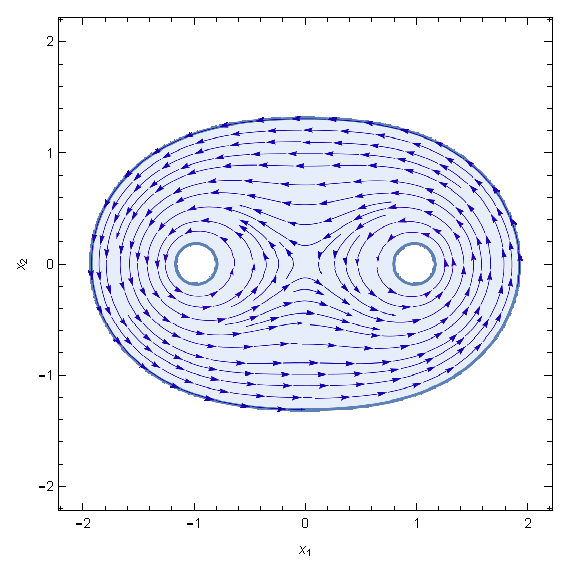
\includegraphics[width=0.6\textwidth]{../Plots/HarmonicVectorFields_gr1.eps}
    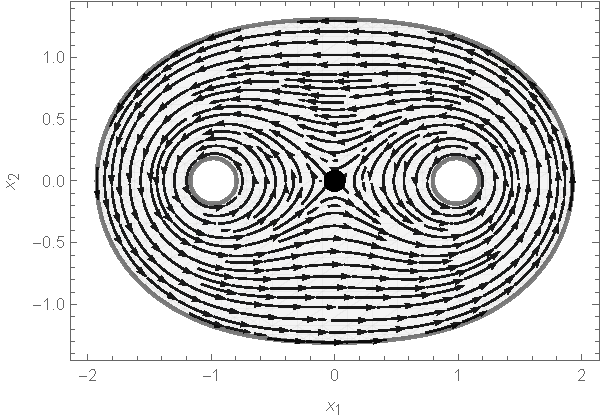
\includegraphics[width=0.9\textwidth]{../Plots/n2_hvf_noInflowNoOutflow_symmetric_gray_2.pdf}
    \caption{A plot of $u=\nabla^\perp\psi$ in the domain $\psi^{-1}\brk*{[-1,1]}$.
      Here $\psi\leftdef\Phi_2\brk*{x-e_1}+\Phi_2\brk*{x+e_1}$.}
    \label{pl:n2_hvf_noInflowNoOutflow}
  \end{figure}
\end{frame}

% \begin{frame}
%   \begin{example}[Stagnation points on the boundary, {\autocite[Ex.\ 6.9]{Koppenhoefer2024}}]
%     Let $X=\overline{B}_4\setminus\brk*{B_1\brk*{2e_1}\cup B_1\brk*{-2e_1}}$ be the domain and let the stream function $\psi$ be given by
%     \begin{equation*}
%       \begin{aligned}
%         \Delta \psi&=0 &&\text{on }\openX\,, \\
%         \psi&=0 &&\text{on the outer ring }4S^1\,, \\
%         \psi&=-1 &&\text{on the left inner ring }S^1(-2e_1)\,, \\
%         \psi&=1 &&\text{on the right inner ring }S^1(2e_1)\,.
%       \end{aligned}\label{eq:n2:hvf:roundRegion:InflowOutflow}
%     \end{equation*} 
%   \end{example}
%   
% \end{frame}

\begin{frame}
  \begin{figure}
    \centering
    % 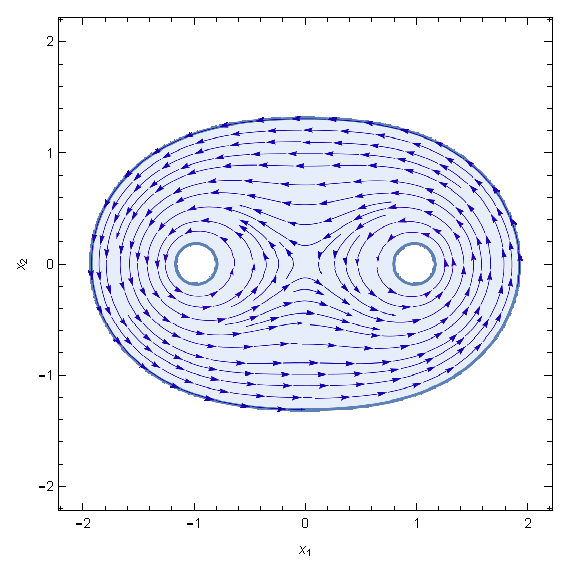
\includegraphics[width=0.6\textwidth]{../Plots/HarmonicVectorFields_gr1.eps}
    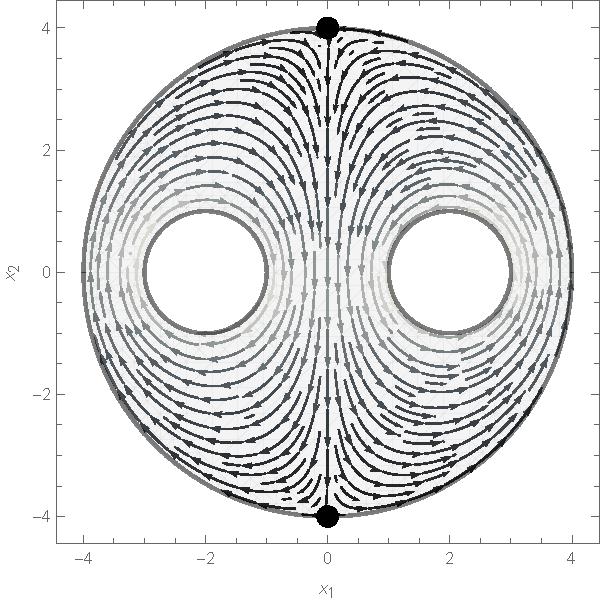
\includegraphics[width=0.6\textwidth]{../Plots/n2_hvf_roundRegion_InflowOutflow_gray_2.pdf}
    \caption{A plot of $u=\nabla^\perp\psi$ in the domain $X$ given as in \autocite[Ex.\ 6.9]{Koppenhoefer2024}.}
    \label{pl:n2_hvf_noInflowNoOutflow}
  \end{figure}
\end{frame}


\begin{frame}
  \begin{proposition}[Condition on the domain topology, {\autocite[Prop.\ 6.11]{Koppenhoefer2024}}]\label{pr:n3_domainCond}
    Let $X$ be a compact orientable odd dimensional manifold with smooth boundary.
    Let further $u\colon X\to TX$ be a smooth vector field with isolated stagnation points on the interior and without
    boundary stagnation points. Then the Euler characteristic of the domain $\chi\brk*{X}=0$ has to vanish.
  \end{proposition} 
\end{frame}

\begin{frame}
  \begin{corollary}[Condition on the type numbers and domain, {\autocite[Cor.\ 6.12]{Koppenhoefer2024}}]\label{co:n3_conditionTypeNbrII}
    Let $X\subset\R^3$ be a compact three-dimensional manifold with smooth boundary and let further
    $u\colon X\to TX$ be a Morse harmonic vector field with no
    inflow or outflow through the boundary. Then
    we have the condition $M_1=M_2$ between the interior type numbers and the Euler characteristic of the domain $\chi\brk*{X}=0$ vanishes.
  \end{corollary}
\end{frame}

\begin{frame}
  \frametitle{Summary}
  \begin{itemize}
    \item Is it possible to have an interior stagnation point and connected entrant and emergent boundaries?
      \begin{itemize}
        \item $d=2$ dimensions: No, unless one allows for holes in the domain
        \item $d=3$ dimensions: Yes and $M_1=M_2$, but not possible for cylinders
        \item $d=4$ dimensions: Yes by a simple example
        \item techniques: Morse theory for manifolds with corners
      \end{itemize}
    \item What is the relation between interior stagnation points and the domain topology for harmonic vector fields without inflow or outflow through the boundary?
      \begin{itemize}
        \item $d=2$ dimensions: $M=-\chi\brk*{X}$
        \item $d=3$ dimensions: $\chi\brk*{X}=0$ and $M_1=M_2$.
        \item techniques: Morse index theorem
      \end{itemize}
  \end{itemize}
\end{frame}


\section{Sources}

\begin{frame}[allowframebreaks]
	\frametitle{Sources}
	\nocite{*}

	% \bibliographystyle{plain}
	\setbeamertemplate{bibliography item}[text]
	% \bibliography{bibliographyFile}
	\printbibliography
\end{frame}

{
  \usebackgroundtemplate{%
  {\transparent{0.6}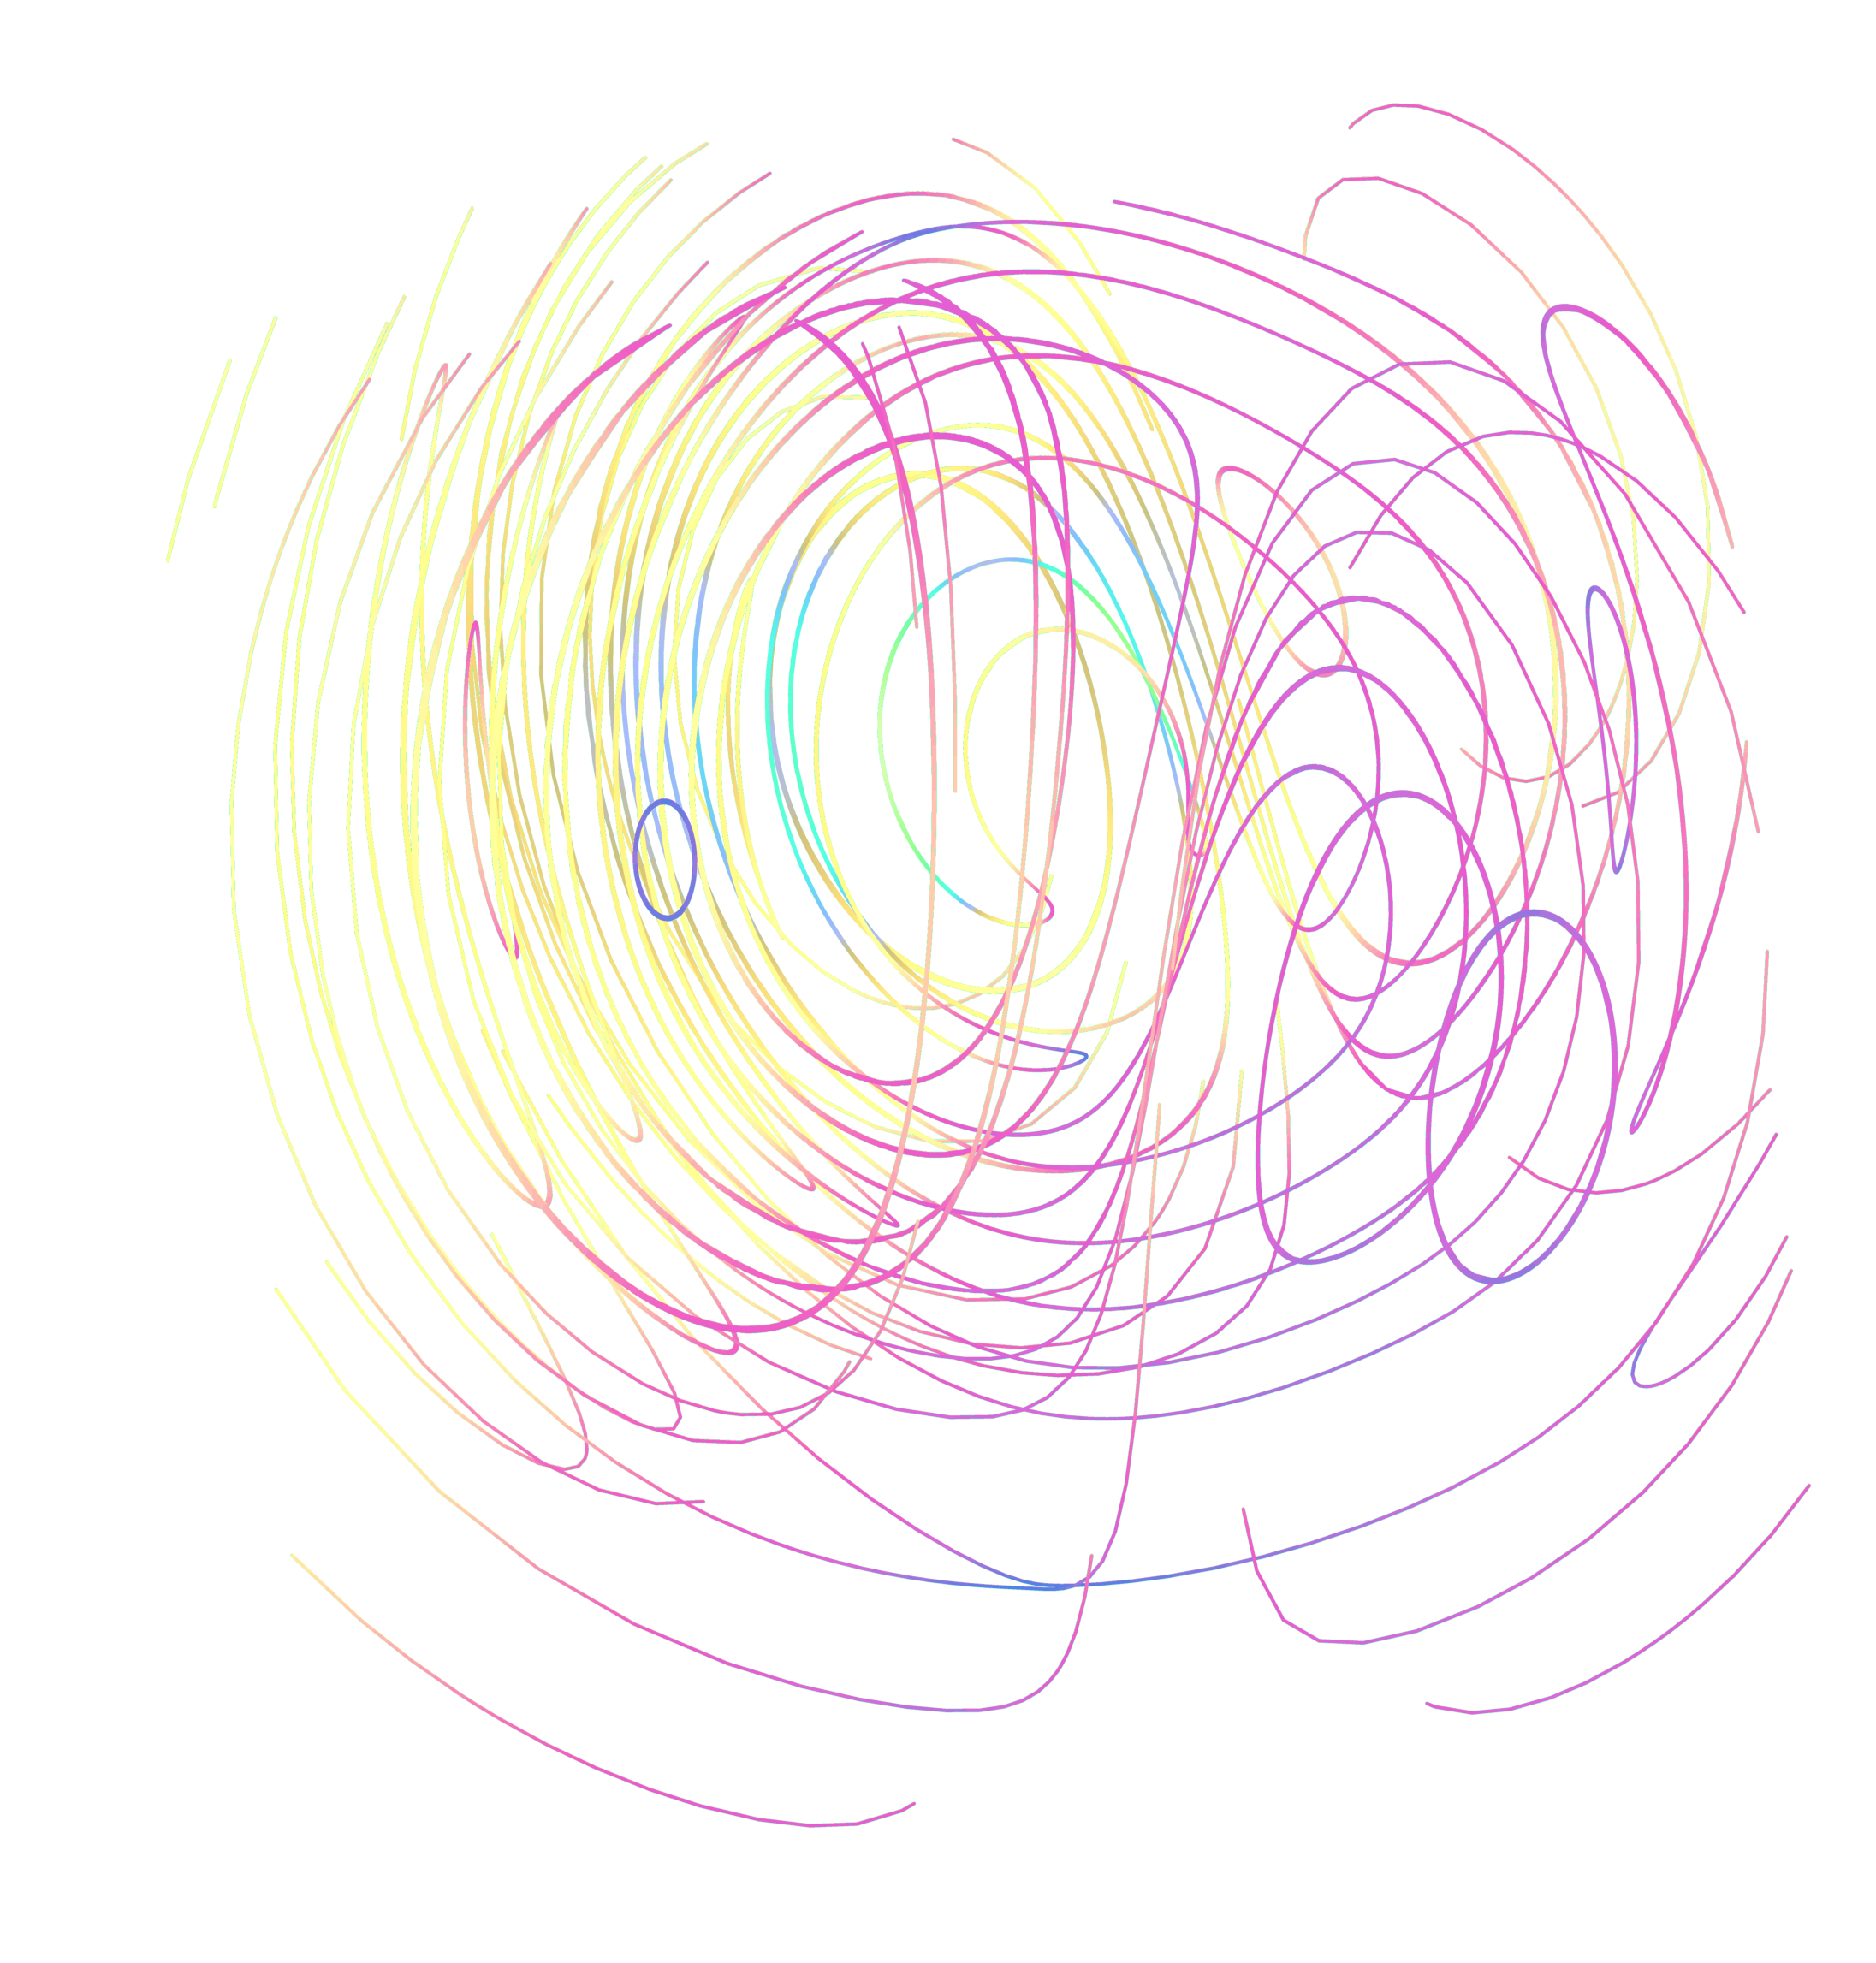
\includegraphics[trim=5cm 3cm 3cm 5cm,width=\paperwidth,height=\paperheight]{../Art/circular_001_colorised.pdf}}}
\begin{frame}[plain]
	\begin{center}
		\Large{{Thank you for your attention.}}
	\end{center}
\end{frame}
}

% \frame[plain]

\end{document}
